\title{ブロックチェーン技術を用いたマネジメント法の提案}
\author{プロジェクトマネジメントコース\\
ソフトウェア開発管理グループ\\
矢吹研究室\\
1442068\\
鈴木 博文}
\date{}
\begin{document}
\maketitle

%本テンプレートの余白は,卒論マニュアルで指示されたものとは違っているが,1ページあたりの文字数は40文字x40行と,卒論マニュアル通りになっている.文字間隔や行間隔を調整して,余白をマニュアル通りにすることもできるが,それでは文章が読みにくくなるため,このような対応をしている.

%\noindent
□□□□□□□□□■□□□□□□□□□■□□□□□□□□□■□□□□□□□□□■
□□□□□□□□□■□□□□□□□□□■□□□□□□□□□■□□□□□□□□□■
□□□□□□□□□■□□□□□□□□□■□□□□□□□□□■□□□□□□□□□■
□□□□□□□□□■□□□□□□□□□■□□□□□□□□□■□□□□□□□□□■
□□□□□□□□□■□□□□□□□□□■□□□□□□□□□■□□□□□□□□□■
□□□□□□□□□■□□□□□□□□□■□□□□□□□□□■□□□□□□□□□■
□□□□□□□□□■□□□□□□□□□■□□□□□□□□□■□□□□□□□□□■
□□□□□□□□□■□□□□□□□□□■□□□□□□□□□■□□□□□□□□□■
□□□□□□□□□■□□□□□□□□□■□□□□□□□□□■□□□□□□□□□■
□□□□□□□□□■□□□□□□□□□■□□□□□□□□□■□□□□□□□□□■
□□□□□□□□□■□□□□□□□□□■□□□□□□□□□■□□□□□□□□□■
□□□□□□□□□■□□□□□□□□□■□□□□□□□□□■□□□□□□□□□■
□□□□□□□□□■□□□□□□□□□■□□□□□□□□□■□□□□□□□□□■
□□□□□□□□□■□□□□□□□□□■□□□□□□□□□■□□□□□□□□□■
□□□□□□□□□■□□□□□□□□□■□□□□□□□□□■□□□□□□□□□■
□□□□□□□□□■□□□□□□□□□■□□□□□□□□□■□□□□□□□□□■
□□□□□□□□□■□□□□□□□□□■□□□□□□□□□■□□□□□□□□□■
□□□□□□□□□■□□□□□□□□□■□□□□□□□□□■□□□□□□□□□■
□□□□□□□□□■□□□□□□□□□■□□□□□□□□□■□□□□□□□□□■
□□□□□□□□□■□□□□□□□□□■□□□□□□□□□■□□□□□□□□□■
□□□□□□□□□■□□□□□□□□□■□□□□□□□□□■□□□□□□□□□■
□□□□□□□□□■□□□□□□□□□■□□□□□□□□□■□□□□□□□□□■
□□□□□□□□□■□□□□□□□□□■□□□□□□□□□■□□□□□□□□□■
□□□□□□□□□■□□□□□□□□□■□□□□□□□□□■□□□□□□□□□■
□□□□□□□□□■□□□□□□□□□■□□□□□□□□□■□□□□□□□□□■
□□□□□□□□□■□□□□□□□□□■□□□□□□□□□■□□□□□□□□□■
□□□□□□□□□■□□□□□□□□□■□□□□□□□□□■□□□□□□□□□■
□□□□□□□□□■□□□□□□□□□■□□□□□□□□□■□□□□□□□□□■
□□□□□□□□□■□□□□□□□□□■□□□□□□□□□■□□□□□□□□□■
□□□□□□□□□■□□□□□□□□□■□□□□□□□□□■□□□□□□□□□■
□□□□□□□□□■□□□□□□□□□■□□□□□□□□□■□□□□□□□□□■
□□□□□□□□□■□□□□□□□□□■□□□□□□□□□■□□□□□□□□□■
□□□□□□□□□■□□□□□□□□□■□□□□□□□□□■□□□□□□□□□■
□□□□□□□□□■□□□□□□□□□■□□□□□□□□□■□□□□□□□□□■
□□□□□□□□□■□□□□□□□□□■□□□□□□□□□■□□□□□□□□□■
□□□□□□□□□■□□□□□□□□□■□□□□□□□□□■□□□□□□□□□■
□□□□□□□□□■□□□□□□□□□■□□□□□□□□□■□□□□□□□□□■
□□□□□□□□□■□□□□□□□□□■□□□□□□□□□■□□□□□□□□□■
□□□□□□□□□■□□□□□□□□□■□□□□□□□□□■□□□□□□□□□■
■■■■■■■■■■■■■■■■■■■■■■■■■■■■■■■■■■■■■■■■
□□□□□□□□□■□□□□□□□□□■□□□□□□□□□■□□□□□□□□□■%文字数チェック用

\tableofcontents%目次

\chapter{序論}
当研究では,急速に発展が拡大するブロックチェーン技術を,プロジェクトマネジメント(以下,PM)学科内の研究室において利用した際の利点・難点を調査する.

ファイナンスとテクノロジーを掛け合わせた造語である「フィンテック」の分野における企業買収や設立が昨年から緩和された\cite{touyou}.中でも世界的に流通が拡大しているのがビットコインを始めとした「仮想通貨」である.これが通貨として機能し,サービスが成り立つために必要な技術がブロックチェーンだ.

ブロックチェーンは「仮想通貨」だけでなく投資や投票など,他の分野でも活用が試みられている.

Jack du Rose氏が運営するColony社は,ブロックチェーンを会社経営・マネジメントに応用し,インターネット上での組織の自律的な運営を試みている\cite{wired}.

\chapter{背景}

\section{ビットコインを始めとした仮想通貨の歴史}
\subsubsection{ビットコインの歴史}
ビットコインは,2008年10月に中本哲史(Satoshi Nakamoto)と名乗る人物がインターネット上に投稿した論文によって,提唱された.

それからわずか3ヶ月後,2009年1月には,ビットコインの理論を実現するためのソフトウェアがオープンソースで開発され,公開された.そしてすぐに,ビットコインの最初の取引が行われた.開発者や,この時からビットコインを所有している人たちは,膨大な価値を持ったビットコインを所有していると言われている.

それからおよそ1年後の2010年2月に,ビットコイン両替が出来る最初の取引所が誕生した.そして同年5月,はじめて現実社会でビットコインを使った決済が行われている.

ビットコインとは,ひとことで言えば「仮想通貨」である.その名の通り「仮想」の「通貨」である.まず「通貨」ということからも,「コイン」ということからも分かる通り,ビットコインはお金である.円やドルというように「お金」であることには変わりない.「お金」なので円やドルのように通貨の単位が存在する.ビットコインの単位は,BTC(ビーティーシー)と表記される.1円や1ドルのように,1BTC(1ビットコイン)と数えることが出来る.

\subsubsection{一般的な仮想通貨の例}
仮想通貨としてイメージしやすいのは,オンラインゲーム内の通貨である.円やドルを支払って,ゲーム内で使われている通貨を手に入れれば,そのゲーム内で使われている通貨が「使える」ゲーム内のお店で,アイテムを買うことができる.ゲーム内でのみ使える,仮想の通貨である.

他にも,特定のWebサイトでのみ使える仮想通貨も存在する.利用登録の際に1,000円で1,000ポイントを購入し,その1,000ポイントで有料サービスを購入するというしくみを利用しているWebサイトが存在する.そのポイントが「使える」Webサイト内でのみ有効な,仮想の通貨である.

\subsubsection{ビットコインと仮想通貨の違い}
仮想通貨とビットコインは何が違うのか.実は存在している理由が全く違うのである.特定のゲームやWebサイト内でのみ使える仮想通貨は,企業単位で作られており,利用者を囲い込むことによって仮想通貨の運営主体が利益を上げることを目標としている.

一方のビットコインは,国家単位で運営されている円やドルと同じく,経済活動を円滑に進めるために作られた仮想通貨なのである.

ビットコインは,世界中で日常生活に「使える」ようにすることを目指して作られている.仮想の通貨なので紙幣や硬貨は存在しないが,代わりにパソコンやスマートフォンをお財布代わりにして,物の売買が実現できるように作られている.

まだまだ発展途上ではあるが,円やドル以上に利便性が高く,安定し,世界中で利用できる次世代の通貨をめざして作られた仮想通貨なのである.

\subsubsection{ビットコインとブロックチェーン}
ビットコインは銀行のような中央を経由せず,直接1対1で通貨のようなものを取引出来る仕組みである.これはつまりサーバークライアントモデルに基づいた信用によらず,取引ができるということである.

この仕組みはP2P(Peer-to-peer)技術と,公開鍵暗号などの暗号技術を用いて実現されている.重要なのは,ネットワーク全体で,特定のどちらかの一方のみを一貫して,正しい取引であると決定できることである.そこでビットコインに導入されたのが「ブロックチェーン」という仕組みである.それぞれの「ブロック」は多数のトランザクションと,あとで説明する「ナンス」と呼ばれる特別な値,そして直前のブロックのハッシュを持っている.「ブロック」に含まれた取引のみを「正しい取引」と認めることにする.そして,ネットワーク全体で「唯一のブロックの鎖」を持つようにする.これによって,一貫した取引履歴を全体が共有できる,というのがブロックチェーンのコンセプトである.

\newpage

\section{ブロックチェーン技術の歴史と応用例}

\subsubsection{ブロックチェーン技術の概要}

ブロックチェーンとは,信頼性,説明責任,透明性を担保しながらビジネス・プロセスを効率化出来る,次世代のトランザクション.アプリケーションの基盤となる技術である.ブロックチェーンはビットコインで有名になった設計パターンだが,その用途にはビットコインにとどまらない可能性がある.ブロックチェーンを活用すれば,これまで全世界のビジネスの根幹を支えてきたビジネス上のやりとりの方法を刷新し,新たなデジタル式のやりとりの方法を構築することができる.ブロックチェーンには,企業間ビジネス・プロセスのコストと複雑性を大幅に削減する可能性がある.分散台帳に基づき低コストで簡単に構築できるビジネス・ネットワーク上で,これまでのような集中管理拠点を設けることなく,価値を持つすべてのモノを追跡,交換できるようになる.

この最新技術が秘めている可能性は,幅広いビジネス・アプリケーションへの応用が期待されている.

たとえば,ブロックチェーンを活用すれば証券の決済にかかる期間を数日から数分に短縮することができる.ほかにも,企業の物流とそれに伴う支払いの管理や,製造メーカー,OEMの委託先メーカー,規制当局間で製造ログを共有して商品のリコール件数を削減するなど,さまざまな用途が考えられる.

\subsubsection{ブロックチェーンの重要な概念}

ブロックチェーンにおける2つの重要な概念は,参加メンバーが価値あるモノを交換する場となるビジネス・ネットワークと,各メンバーが所有し,メンバー間で常に内容が同期される台帳である.

ビジネス・ネットワークは複数のノードで構成される分散型P2Pアーキテクチャで,各ノードは市場の参加者である.これはプロトコルを共有する複数のピアがタランザクションを検証しコミットすることで合意を形成する.

共有台帳はブロックチェーン上で取引を行う企業に正しい情報を提供する唯一の機能である.ビジネス・ネットワーク上の全てのトランザクションを記録し,参加者間で共有される.各参加者に複製され,それぞれの参加者が独自にコピーを所有するが,自分が許可されたトランザクションしか参照できない.

\newpage

\subsubsection{ブロックチェーン技術の応用事例}

ブロックチェーンは,仮想通貨以外への応用が始まっている.ブロックチェーンを応用し,送金や証券などの金融取引や資産管理をはじめとし,ポイントや公共サービスなどでも活用しようとする動きがある.

米Nasdaq社の未公開株式取引市場であるNasdaq Private Marcketの「Nasdaq Linq」は,株式未公開企業の従業員らが,自身で保有している株式を売買でき,その取引の「台帳」を実装する技術としてブロックチェーンを使用しているのだ.

金融以外の分野では米Gyft Block社がブロックチェーンを活用して,ポイント交換システムを立ち上げており,安価で信頼性の高い,ギフトカードを交換する仕組みを作り出している.

また,豪Flux社が政治に活かそうと選挙システムを構築するほか.英Everledger社はダイヤモンドの形状をセンサーで読み取りデジタル指紋に変換し,ブロックチェーンにダイヤモンドの認定書を記録する.そのダイヤモンドが消費者に販売されるまでの取引ルートを追跡してブロックチェーンに記録することにより,消費者が盗品を購入してしまうことを防いでいる.

上記以外にも,不動産取引・食品管理・農業支援・個人特定・履歴書管理など金融部門のみに限らず様々な分野での応用が進んでおり,ブロックチェーン技術の活用は今後さらに拡大が発展していくと考えられる.

\newpage

\section{Colony社によるブロックチェーン技術の応用例}

Colony創業者兼最高経営責任者であるJack du Rose(ジャック・デュ・ローズ)氏は分散型ネットワークを活用し,インターネット上に存在する組織を自立分散的に運営することで注目を集めている.もともとは宝石デザイナーとして活躍していた.

Colony社\cite{colony}の経営は,一言で言えば,分散型のプラットフォームであり,ブロックチェーンを活用することで,インターネット上での組織の自律的な運営を可能にするものである.

「信用」「信頼」「価値」を分散型で担保するオープンなプラットフォームであるColonyは,分散型の企業や非営利組織の概念を提唱しており,「会社」のあり方そのものを買えうる可能性を秘めている.

それは「ソーシャルコラボレーションプラットフォーム」と言い換えることも可能だ.利用方法としてはたとえば「Webサイトをつくりたい」と考えたとき,そのWebサイトを作るための「Colony」を立ち上げ,デザイナーやエンジニアなど参加者を募るというもの.「Colony」に参加するか,立ち上げるか.このどちらかで利用できる.

これだけ聞くとクラウドソーシングを思い浮かべるが,大きく違うのは,その対価・報酬と意思決定のあり方だ.自律分散型のガバナンスの重要性を指摘するデュ・ローズは,フリーランスをマネジメントするための方法として「ブロックチェーン」が有効だと指摘する.ジョブのアサイン,組織の意思決定に分散型ネットワークを活用するというわけだ.つまり参加者同士が直接つながり,提案と投票によって意思決定がなされる.その「Colony」への貢献度に応じ,民主的に評価される真にフラットな組織を志向する.

デザインやプログラミングといった作業への対価は,Colony内の独自のトークンで支払われる.トークンは企業や株式のように「Colony」の所有権を表すもので,現金と取引することができる.

\chapter{目的}

ブロックチェーン技術を,マネジメントに応用した例を参考に,PM学科内の研究室において同技術を利用した際の利点・難点を研究する.出欠情報・プロジェクト内での作業時間・成績情報・経歴情報など,存在証明が必要とされるドキュメントを管理するプロトタイプを実装し記録改ざんの複雑化と存在証明の効率化を図る.

\chapter{手法}

\section{ソフトウェアの導入}

本研究において,いくつかのソフトウェアを利用する.Windows用ソフトウェアパッケージ管理ソフトであるChocolateyを始めとし,仮想環境を構築するために利用されるVagrant,VirtualBox,LinuxOSであるUbuntu16.04 LTSについても解説を行う.

研究内では,ブロックチェーンの基本的な概念を理解するためにNaiveChainを用い,その後ブロック作成に関する契約行動を自動実行出来る,スマート・コントラクトが構築可能なEthereumを利用する.ブロックチェーンについての基本実装についてはこの2つのソフトウェアについて解説を行う.

\newpage

\subsection{Chocolatey}

Chocolatey\cite{chocolatey}はWindowsのコマンドライン上で利用することができる,Windows用のパッケージマネージャである.Linuxで用いられるapt-getやyumのようなパッケージ管理コマンドと同様に使用を行うことができる.図\ref{chocolatey}はChocolateyの公式ホームページである.

Chocolateyは,バージョン管理と依存関係の両方の要件を理解しているパッケージフレームワークを利用して,Windowsソフトウェアの管理のあらゆる側面を容易に処理できるように設計された単一の統一されたインターフェイスである.

Chocolatey本体のインストールはコマンドプロンプト(管理者権限)を起動し以下のスクリプトを入力し実行する.

\begin{verbatim}
@"%SystemRoot%\System32\WindowsPowerShell\v1.0\powershell.exe" -NoProfile 
-InputFormat None -ExecutionPolicy Bypass -Command "iex ((New-Object 
System.Net.WebClient).DownloadString('https://chocolatey.org/install.ps1
'))" && SET "PATH=%PATH%;%ALLUSERSPROFILE%\chocolatey\bin"
\end{verbatim}

\begin{figure}[htb]
\centering
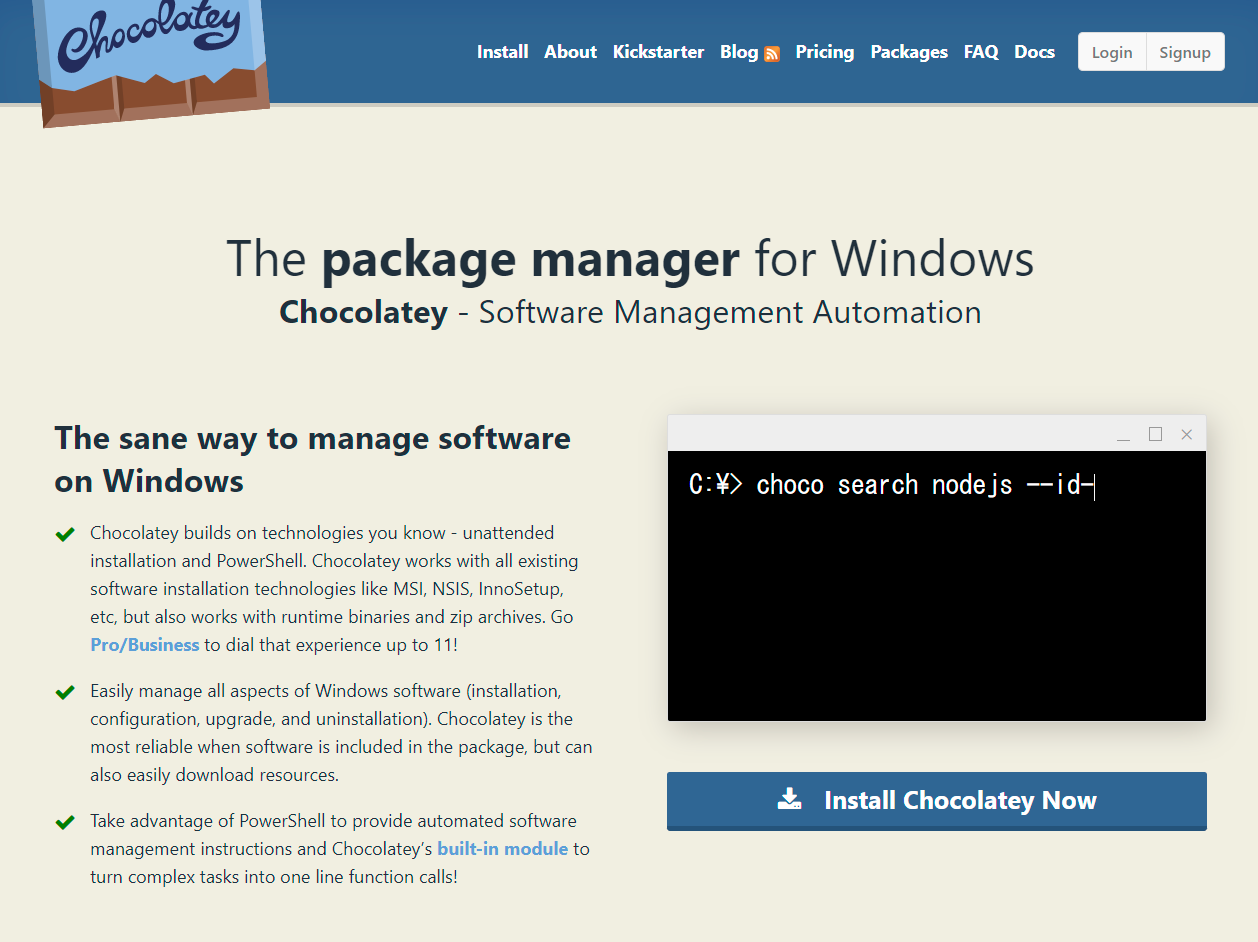
\includegraphics[width=12cm]{images/chocolatey.png}
\caption{Chocolateyの公式ホームページ}\label{chocolatey}
\end{figure}

\newpage

インストール完了後は\texttt{choco install [packageName]}などとして任意のパッケージをインストールする.\texttt{choco install [packageName1] [packageName2] ...}とすると複数コマンドを一括してインストールできるほか,\texttt{-y}を追加することによりインストールへの同意を一括してYesとすることが出来る.研究において利用する主なコマンドの一覧を表\ref{table:Chocolatey}として下記に記載する.

\begin{table}[htb]
\caption{Chocolateyで使用できるコマンド}
\label{table:Chocolatey}
\begin{tabular}{|p{5cm}|p{7.5cm}|} \hline
choco install [packageName] & 指定パッケージをインストールする.\\ \hline
choco list & インストール可能なパッケージの一覧を表示する.\\ \hline
choco list -lo & インストール済みのパッケージ一覧を取得する.\\ \hline
choco update [packageName] & 指定パッケージをアップデートする.\\ \hline
choco update all & インストール済みの全てのパッケージをアップデートする.\\ \hline
choco uninstall [packageName] & 指定パッケージをアンインストールする.\\ \hline
\end{tabular}
\end{table}

当研究で利用するソフトウェアは以下のコマンドをChocolateyで実行することで導入できる.図\ref{clist}はローカルにインストールされたソフトウェアの一覧を表示した結果である.

\texttt{choco install vagrant VirtualBox git rsync -y}

\begin{figure}[htb]
\centering
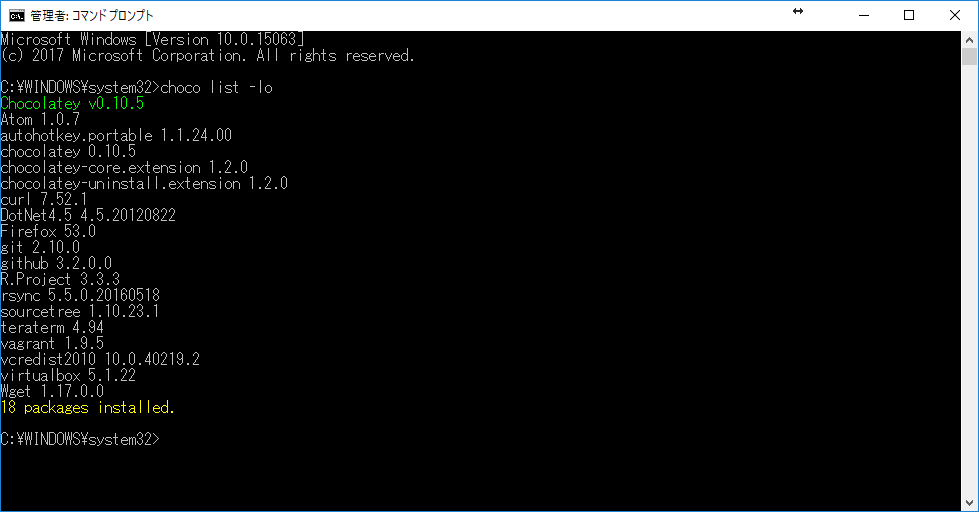
\includegraphics[width=12cm]{images/clist.png}
\caption{Chocolateyを用いて導入したソフトウェア一覧の表示}\label{clist}
\end{figure}

\newpage

\subsection{VirtualBox}

VirtualBox\cite{VirtualBox}はx86ベース・システム用の強力なクロスプラットフォーム仮想化ソフトウェアである.「クロスプラットフォーム」とは,Windows,Linux,Mac OSXさらにSolaris x86コンピュータにインストール可能であることを意味する.また,「仮想化ソフトウェア」とは,同じコンピュータ上で同時に複数のOSを実行する複数の仮想マシンを生成,実行できることを意味する.たとえば,Mac上でWindowsとLinuxを実行したり,Windows PC上でLinuxとSolarisを実行したり,Linuxシステム上でWindowsを実行したりすることができる.以下にVirtualBoxを利用するにおいて用いられる主な用語の説明を記載する.

\subsubsection{ハードウェアシュミレーション}
ハードウェアによる仮想化支援機能としてVT-xと,AMD-Vへの対応を含む.対応当初はデフォルトでどちらも有効となっていなかったが,現在のバージョンで提供される機能の一部には,これらの仮想化支援機能を必要とするものがある.バージョン5.0よりKVMが選択可能になり,Linuxにおいてハードウェアエミュレーションのオーバーヘッドが削減可能になった.

\subsubsection{ハードディスク}
ハードディスクドライブは,通常「仮想ディスク・イメージ(Virtula Disk Images)」と呼ばれる他の仮想化ソリューションとは互換性のない特別なコンテナ・フォーマットとしてエミュレートされる.これらは,ホストOS上のシステムファイル(拡張子.vdi)として格納される.別の方法として,VirtualBoxはiSCSIの対象との接続が可能で,それらを仮想ハードディスク群として使用することが出来る.この他,他の仮想マシンソフトウェアで用いられる,vmdk(VMware),vhd(Microsoft Virtual PC),hdd(Parallels)などの仮想ディスクイメージにも対応する.ただし,これらのディスクイメージは本来VirtualBox向けのフォーマットではない為,フォーマットのバージョンとVirtualBoxのバージョンの対応など,利用に当たっては互換性の面における注意が必要であるが,有志によりコンバートユーティリティがいくつか開発されている.

\subsubsection{光学ドライブ}
CDやDVDドライブとしてISOイメージが使用できる.例えば,LinuxディストリビューションのDVDイメージをダウンロードして,直接VirtualBoxで使用することが出来る.その場合,ISOイメージをCD-RやDVD-RWといった物理メディアに焼き込む必要がない.また,物理的ディスクを仮想マシンから直接的にマウントすることも可能である.

\newpage

\subsubsection{ネットワーク機能}
イーサネット・アダプタとして,AMD PCnet-PCI Ⅱ(Am79C970A),AMD PCnet-FAST Ⅲ(Am79C973),Intel PRO/1000 MT Desktop(82540EM),Intel PRO/1000 T Server(82543GC),Intel PRO/1000 MT Server(82545EM)のいずれかを仮想化する.これらの仮想化されたアダプタによる外部との接続手段として,NAT(ホストOSによるNAPT機能),ブリッジアダプタ(ホストOSの物理インターフェースとのブリッジ機能),内部ネットワーク(ゲストOS同士を接続する内部的なネットワーク),ホストオンリーアダプタ(ホストOS上の仮想Ethernetアダプタと直接的に接続する)が提供される.新規作成されるマシンは,いずれかのアダプタとNATの組み合わせが設定される.ゲストOS上のアプリケーションは,これによりホストOSを経由して外部との通信が可能となる.NATを提供するホストOSは,一般的なブロードバンドルータと同様の動作を行う.バージョン5.0から準仮想化機能が搭載され始め,準仮想化ネットワークが選択可能になった.この仮想ネットワークインターフェースを利用することで,VirtualBoxがvirtio-netのドライバを持つOSのカーネルと協調してVirtualBox上のゲストOSと物理ネットワークインターフェースの間で直接データを受け渡しすることが可能になり,ネットワークにおけるエミュレーションのオーバーヘッドを削減することが可能になる.

図\ref{VirtualBox}はVirtualBoxの起動画面である.

\begin{figure}[htb]
\centering
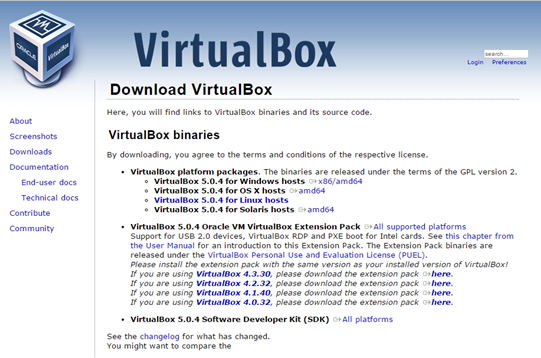
\includegraphics[width=12cm]{images/VirtualBox.png}
\caption{VirtualBoxの起動画面}\label{VirtualBox}
\end{figure}

\newpage
 
\subsection{Vagrant}

Vagrant\cite{vagrant}は,FLOSSの仮想開発環境構築ソフトウェアである.VirtualBoxをはじめとする仮想化ソフトウェアやChefやSalt,Puppetといった構成管理ソフトウェアのラッパーとみなすこともできる.

Vagrantを用いると,構成情報を記述した設定ファイルをもとに,仮想環境の構築から設定までを自動的に行うことが出来る.通常の仮想化ソフトウェアでは環境構築のために複雑なコマンド操作を行うが,Vagrantでは数行のコマンドで構築が完了する.Vagrantfileというテキストファイルで仮想マシンの構成を管理しており,ファイル内に仮想マシン起動に構成管理ツールを実行するよう指定する箇所がある.このVagrantfileと構成管理ツールの設定ファイルを共有することで,どこでも同じ仮想マシンを再現することができるようになる.以下にVagrantを利用するにおいて用いられる主な用語の説明を記載する.

\subsubsection{Boxファイル}

仮想マシン起動時にテンプレートとなるイメージファイルであるが,一般的なISOイメージファイルとは異なる.
Boxファイルの一覧はhttps://atlas.hashicorp.com/searchに公開されている.同サイトからBoxファイルを取得して利用するほか,自身でBoxファイルを作成することも可能である.

\subsubsection{Vagrantfile}

仮想マシンに構成を記述するファイル.主に以下の項目を指定する.

\begin{itemize}
\item 起動する仮想マシンの指定
\item ネットワークの設定
\item 共有フォルダの設定
\item CPUやメモリの割当などマシンスペックの設定
\item Shellや構成管理ツールの実行を指定するプロビジョニング
\end{itemize}

\subsubsection{プロバイダ}

仮想化ソフト,いわゆる仮想環境のこと.VagrantではディフォルトでVirtualBoxをサポートするが,プラグインをインストールすればVMwareやParallels,AWS(EC2)などにも対応可能である.

\subsubsection{プロビジョニング}

ミドルウェアのインストールや設定を行うツール.ここではShellや構成管理ツール(Chef,Puppet,Ansible)のことを指す.Vagrantfile内で指定し,呼び出す.本研究ではprovision.shとしファイルを作成する.

\subsubsection{共有フォルダ}

ローカルと仮想マシンの間でファイルを同期する機能のこと.ディフォルトでは,ローカルのVagrantfileがあるフォルダと仮想マシンの\texttt{\$/vagrant}が同期されている.他のフォルダを指定したい場合はVagrantfileの\texttt{config.vm.synced\_folder}に指定する.

\subsubsection{プラグイン}

\texttt{vagrant plugin install}で後からインストール可能な追加機能.

\subsubsection{コマンド一覧}

Vagrantにおいて使用される頻度の高いコマンドを表\ref{table:Vagrant}に記載する.

\begin{table}[htb]
\caption{Vagrantで使用できるコマンド}
\label{table:Vagrant}
\begin{tabular}{|p{5cm}|p{7.5cm}|} \hline
vagrant box add <name> & Boxを追加する.\\ \hline
vagrant box remote <name> & Boxを削除する.\\ \hline
vagrant box list & Boxの一覧を表示する.\\ \hline
vagrant init [name] & Vagrantfileの作成をする.\\ \hline
vagrant up & 仮想マシンを起動する.\\ \hline
vagrant halt & 仮想マシンを停止する.\\ \hline
vagrant reload & 仮想マシンを再起動する.\\ \hline
vagrant destroy & 仮想マシンを削除する.\\ \hline
vagrant package & 仮想マシンをBox形式で出力する.\\ \hline
vagrant plugin install <name> & プラグインを追加する.\\ \hline
vagrant plugin list & プラグイン一覧を表示する.\\ \hline
\end{tabular}
\end{table}

上記以外のVagrantで利用できるコマンドは\texttt{vagrant -h}で確認ができる.すべてのコマンドは\texttt{-h}オプションを付けて実行(例 \texttt{vagrant up -h})することで,各コマンドの詳細なヘルプが表示される.

\newpage

\subsubsection{研究用仮想マシンの構築}

本研究においては所属研究室である,矢吹研究室の公式仮想マシンを利用して開発を行う.研究室公式仮想マシンのベースとなるBoxファイル,プロビジョニングを作成する時点からの解説を行う.

まず,Guest Additionを更新し,ディスクサイズの変更を簡易化するためのプラグインを導入する.
\begin{verbatim}
vagrant plugin install vagrant-vbguest
vagrant plugin install vagrant-disksize
\end{verbatim}

Cドライブ上にVagrant専用のディレクトリを作成する.
\begin{verbatim}
cd :
cd /
mkdir vagrant
cd vagrant
git clone https://github.com/yabukilab/machine.git
\end{verbatim}

研究室外やVagrantfileを初期設定で利用したい場合などはBoxファイルを直接利用する.特に制限がなければUbuntuの最新OSであるUbuntu16.04 LTS(ubuntu/xenial64)を利用する.

\begin{verbatim}
mkdir ubuntu
cd ubuntu
vagrant init ubuntu/xenial64
\end{verbatim}

\newpage

Vagrantfileをテキストエディタ等で開き,下記スクリプトが有効であることを確認する.Boxを取得した際に記載されているスクリプトはコメントアウトを外し,記載がないものは下記を参考に追加する.

\begin{verbatim}
Vagrant.configure(2) do |config|
  config.vm.box = "ubuntu/xenial64"
  if Vagrant.has_plugin?("vagrant-disksize")
    config.disksize.size = "10GB"
  end
  config.vm.network:forwarded_port, guest: 80, host: 80
  config.vm.network:forwarded_port, guest: 443, host: 443
  config.vm.network:forwarded_port, guest: 5432, host: 5432
  config.vm.network:forwarded_port, guest: 8888, host: 8888
  config.vm.synced_folder "./html", "/var/www/html"
  config.vm.provider "VirtualBox" do |vb|
    vb.memory = "4096"
    vb.cpus = 2
  end
  config.vm.provision "shell", path: "provision.sh"
  config.vbguest.auto_update = false
end
\end{verbatim}

\newpage

Vagrantfileがあるディレクトリと同階層上にprovision.shを作成し下記スクリプトを記載する.2行目は研究室にあるパッケージのキャッシュサーバを利用するための設定のため,研究室外で使うときは,この行を削除する.

\begin{verbatim}
#Timezone
timedatectl set-timezone Asia/Tokyo

echo 'Acquire::http::Proxy "http://10.100.192.4:3142/";' > 
/etc/apt/apt.conf.d/02proxy

apt update

echo "alias ls='ls -F'" >> /home/ubuntu/.bashrc
echo "alias R='R --no-save'" >> /home/ubuntu/.bashrc
echo "alias jn='jupyter notebook --no-browser --ip=0.0.0.0'" >> 
/home/ubuntu/.bashrc
chown ubuntu:ubuntu /home/ubuntu/.bashrc

echo '. ~/.bashrc' >> /home/ubuntu/.bash_profile
echo 'export PATH="$HOME/anaconda3/bin:$PATH"' >> 
/home/ubuntu/.bash_profile
chown ubuntu:ubuntu /home/ubuntu/.bash_profile

echo "options(repos = 'https://cloud.r-project.org/')" >> 
/home/ubuntu/.Rprofile
chown ubuntu:ubuntu /home/ubuntu/.Rprofile
\end{verbatim}

\newpage

\texttt{vagrant up}を実行し仮想マシンを起動する.
VirtualBox以外で利用する場合は\texttt{vagrant up --provider virtulabox}とする必要があるがディフォルトのプロバイダがVirtualBoxの場合は特に指定する必要はない.指定したBoxが登録されていない場合は,自動的にダウンロードしてBoxを追加(\texttt{vagrant box add})を行う.\\

仮想マシンが起動したら\texttt{vagrant ssh}としてWindowsのコマンドプロンプトからsshログインを行う.図\ref{cmd}はその実行結果である.

\begin{figure}[htb]
\centering
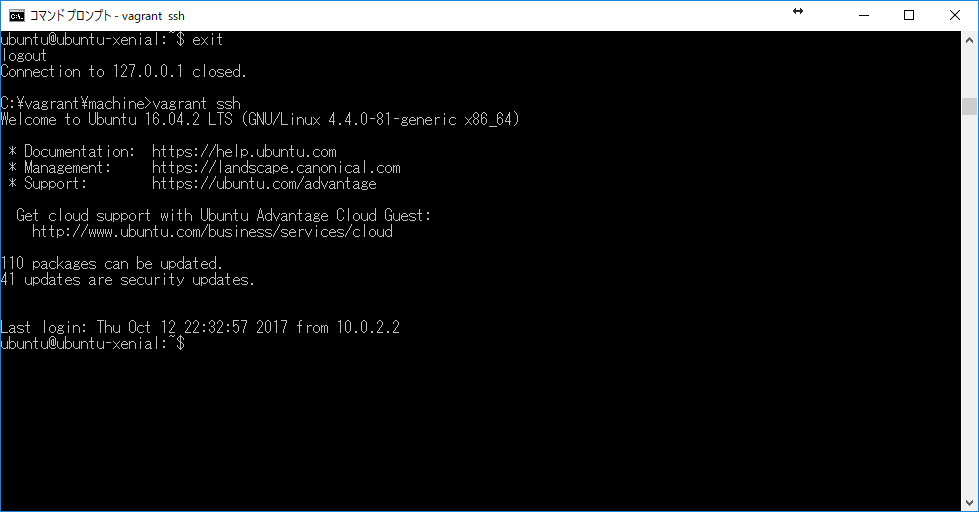
\includegraphics[width=12cm]{images/vagrant.png}
\caption{コマンドプロンプトからssh接続で表示した起動画面}\label{cmd}
\end{figure}

\newpage

PuTTYやTeraTermなどのSSHクライアントを使用してログインすることも出来る.接続先ホスト名は127.0.0.1,接続先ポートは2222を指定する.ユーザ名は\texttt{ubuntu}パスワードは\texttt{C:\textbackslash Users\textbackslash<username>\textbackslash.vagrant.d\textbackslash boxes\textbackslash ubuntu-VAGRANTSLASH-xenial64
\textbackslash20XXMMDD.0.0\textbackslash VirtualBox\textbackslash Vagrantfile}に記載がある.パスワードは\texttt{passwd}として任意に変更できるため,必要に応じて変更する.図\ref{tera}はその起動画面である.

\begin{figure}[htb]
\centering
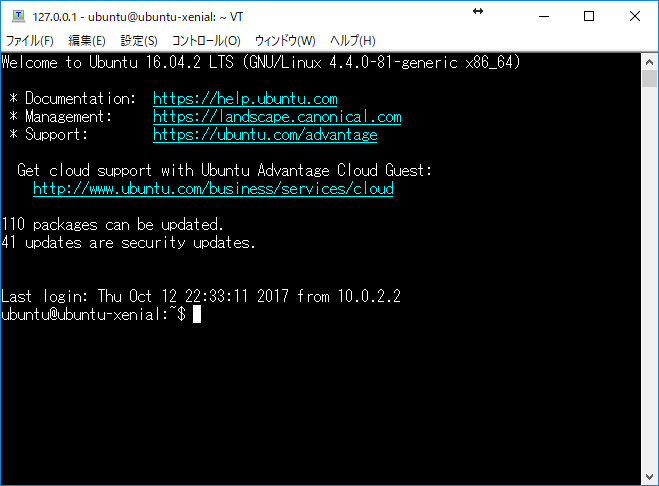
\includegraphics[width=12cm]{images/teraterm.png}
\caption{TeraTermからssh接続で表示した起動画面}\label{tera}
\end{figure}

\newpage

\subsection{Ubuntu}

Ubuntu\cite{ubuntu}はコミュニティにより開発されているオペレーティングシステムである.ラップトップ,デスクトップ,そしてサーバーに利用することが出来る.Ubuntuには,家庭・学校・職場で必要とされるワープロやメールソフトから,サーバーソフトウェアやプログラミングツールまで,あらゆるソフトウェアが含まれている.

Ubuntuは現在,そして将来的に渡って無償で提供されている.ライセンス料を支払う必要はない.Ubuntuをダウンロードすれば,友人や家族と,あるいは学校やビジネスに,完全に無料で利用できる.

Ubuntuは,セキュリティに配慮して設計されています.デスクトップおよびサーバーの無償セキュリティアップデートが,少なくとも9ヶ月間に渡って提供される.長期サポート(LTS)版を利用すれば,5年間に渡りセキュリティアップデート提供される.もちろん,LTS版を利用するために追加の費用は必要ない.図\ref{ubuntu}はUbuntu Desktopの起動画面である.

\begin{figure}[htb]
\centering
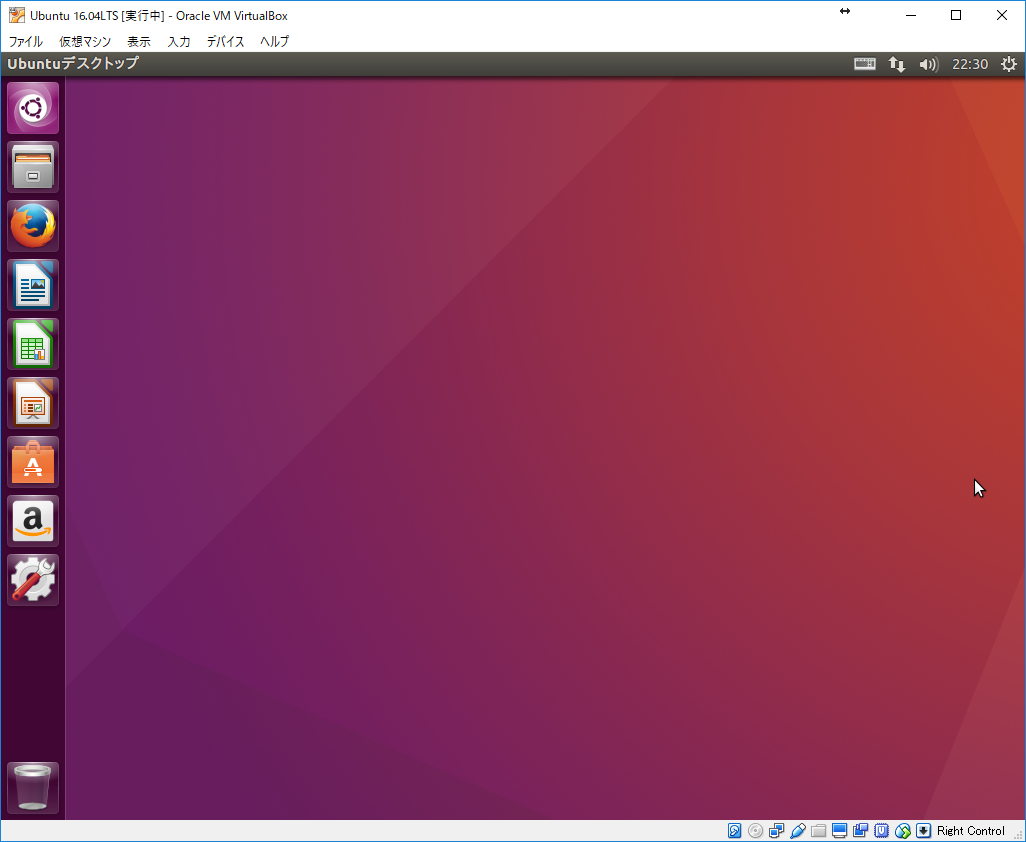
\includegraphics[width=12cm]{images/ubuntu.png}
\caption{Ubuntu Desktopの起動画面}\label{ubuntu}
\end{figure}

\newpage

\subsection{Docker}

Docker\cite{docker}はもともと,DotCloud社(現 Docker Inc.)が開発者やIT部門をターゲットとしたアプリケーションやOSの開発・配備を行うための基盤ソフトウェアとして開発され,2013年にリリースされた.このソフトウェアは,オープンソースソフトウェアの「Docker」として公開され,その使い勝手の良さから,多くの開発y差,IT部門の管理者で瞬く間に利用されることになった.Dockerは,仮想化ソフトウェアに比べ,極めて集約度の高いITシステムを実現することができる.

Dockerは,高性能なアプリケーションの開発・実行環境の提供だけでなく,それらのOSやアプリケーションを世界中で共有し,ITシステムがある目的を達成するために必要な工程を自動化するサービスを提供する点が革新的と言える.世界中の開発者やIT部門のシステム管理者が共通して理解できる同じITシステムを使えば,他者が作ったシステムを少し変える,または,そのまま使うことで,開発,システムテスト,実システムへの配備の工数を大幅に削減することができるようになる.具体的には,例えば,Webアプリケーションの開発において,その動作に必要となるライブラリや,起動,停止,監視用のスクリプトを新たに調査・別途開発するといった“追加の作業”を極力おさえることができる.

\begin{table}[htb]
\caption{Dockerで使用できるコマンド}
\label{table:Vagrant}
\begin{tabular}{|p{5cm}|p{7.5cm}|} \hline
docker pull <imagename> & イメージを参照してくる.\\ \hline
docker build --no-cache=true & キャッシュを無効にする.\\ \hline
docker run -h example -i -t <imagename> /bin/bash & ホスト名(例:example)を付けて起動する.\\ \hline
docker run -name example -i -t <imagename> /bin/bash & コンテナ名(例:example)を付けて起動する.\\ \hline
docker start -a <Contaner ID> & コンテナを起動してログインする.\\ \hline
docker attach <Contaner ID> & 起動中のコンテナにログインする.\\ \hline
docker ps & 起動中のコンテナの一覧を表示する.\\ \hline
docker images & イメージの一覧を表示する\\ \hline
docker rmi <Image ID> & イメージを削除する.\\ \hline
\end{tabular}
\end{table}

\newpage

\subsubsection{Dockerの導入}

仮想環境内にDockerを導入するために以下の手順を実行する.

\begin{enumerate}
\item 管理者でないコマンドプロンプトを起動し\texttt{cd /vagrant/machine}などとして仮想環境のあるディレクトリへ移動する.
\item \texttt{vagrant up}を実行し\texttt{vagrant ssh}で仮想環境へssh接続する.
\item \texttt{sudo apt-get update}を実行し,aptのアップデートを行う.
\item \texttt{sudo apt install docker.io -y}としDockerの導入を行なう
\item \texttt{docker -v}と入力後実行し,図\ref{docker}のようにバージョン確認ができれば導入は完了である.なお,執筆時点でのバージョンは1.13.1である.
\end{enumerate}


\begin{figure}[htb]
\centering
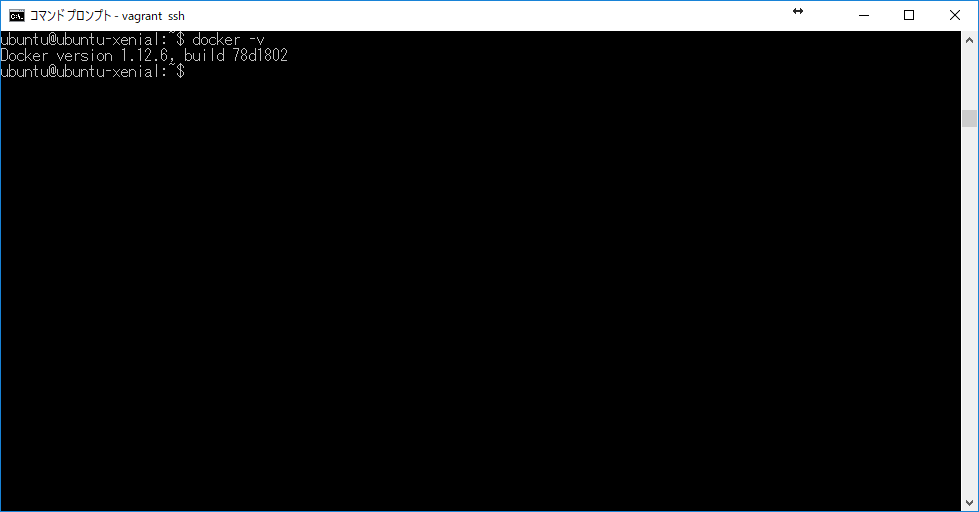
\includegraphics[width=12cm]{images/docker.png}
\caption{Dockerの起動画面}\label{docker}
\end{figure}

\newpage

\subsubsection{Docker Compose}
複数のコンテナを組み合わせた構成でサービスを運用している場合,コンテナに対し特定のパラメータを指定したり,特定の順序での起動が必要となるケースがある.こういった作業を自動化するツールが,「Docker Compose」だ.

Docker ComposeはDockerが開発するコマンドラインツールで,あらかじめ用意しておいた設定ファイルに従ってコンテナを起動するツールだ.設定ファイルには複数のコンテナに関する記述が可能で,コンテナの起動オプションやコンテナに与える環境変数など,さまざまな設定も同時に記述できる.また,コンテナ同士の依存関係を設定することも可能で,これによって関連するコンテナを複数まとめて起動することも可能だ.

この場合,設定された依存関係に応じて適切な順番でコンテナが起動されるようになっており,コマンド1つで簡単に必要なサービスを開始できるようになっている.逆にコンテナを停止させる際も,自動的に適切な順番でコンテナを停止させるようになっている.またDocker Swarmとの統合機能も提供されており,コンテナを複数実行させる(スケールさせる)操作も可能だ.コンテナの実行だけでなくビルド操作もサポートされている.

\begin{itemize}
\item build

サービスのビルドを実行する.サービスとは「Web」や「DB」を指し,ymlファイルにimageの情報がある場合でローカルにそのイメージ名がなければリモートからプルしてくる.

\item config

docker-compose.ymlで書かれている内容が表示される.

\item exec

docker execコマンドと同等のことができる.引数にサービス名と実行するコマンドを指定して実行する.

\item images

対象のイメージの情報を表示する.

\item kill

コンテナを強制停止する.

\item ps

コンテナの一覧を表示する.docker psでも表示される.

\item run

引数で指定したサービスのコンテナ内でコマンドを実行する.

\item start

サービスを開始する.既にコンテナがある状態でのみ実行できる.

\item stop

サービスを停止する.

\item up

コンテナを作成して,起動する.\texttt{-d}をつけることでバックグラウンドで実行することができる.また\texttt{--build}をつけることで起動前にイメージも構築する.
\end{itemize}

\subsubsection{Docker-Composeの導入}

仮想環境内にDocker-Composeを導入するために以下の手順を実行する.

\begin{enumerate}
\item 管理者でないコマンドプロンプトを起動し\texttt{cd /vagrant/machine}などとして仮想環境のあるディレクトリへ移動する.
\item \texttt{vagrant up}を実行し\texttt{vagrant ssh}で仮想環境へssh接続する.
\item \texttt{sudo apt-get update}を実行し,aptのアップデートを行う.
\item \texttt{sudo apt install docker-compose -y}としDockerの導入を行なう
\item \texttt{docker-compose -v}と入力後実行し,図\ref{docker-compose}のようにバージョン確認ができれば導入は完了である.なお,執筆時点でのバージョンは1.8.0である.
\end{enumerate}

\begin{figure}[htb]
\centering
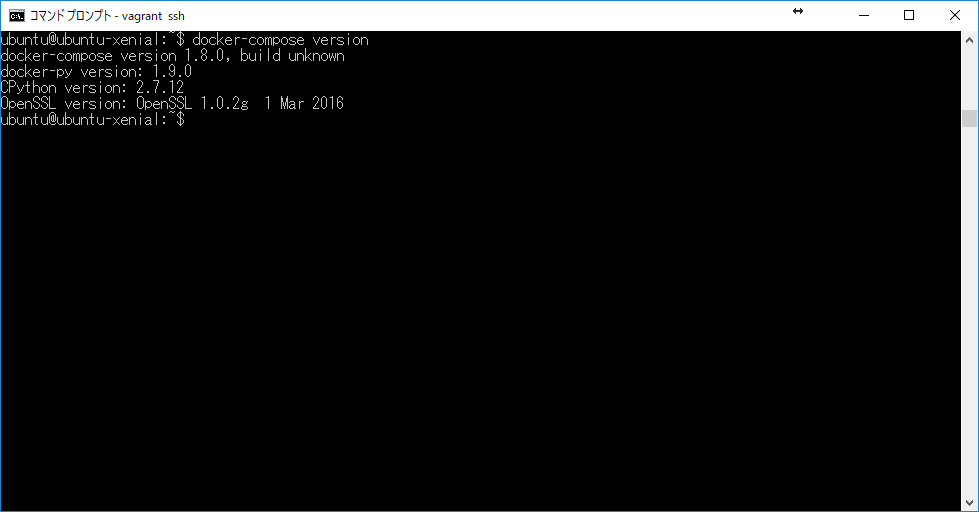
\includegraphics[width=12cm]{images/docker-compose.png}
\caption{Docker Composeの起動画面}\label{docker-compose}
\end{figure}

\newpage

\subsection{NaiveChain}\label{addnaivechain}

ブロックチェーンは基本的な概念は非常にシンプルである.分散型データベースで,順序付けられたレコードのリストが連続的に増加していく.しかしシンプルとは言え,ブロックチェーンやそれを使うことで解決しようとしている問題について話をする際にボトルネックとなることがある.

そのため,本来シンプルであるべきブロックチェーンの理解がより困難になってしまっている.抜け目のないソースコードであれば尚更である.そこで開発されたのがLauri Hartikka氏によるNaiveChain\cite{naivechain}である.このソフトウェアは200行のJavaScriptによって実装された,非常にシンプルなブロックチェーン作成ソフトウェアである.

以下の手順で導入とその確認を行なう.

\begin{enumerate}
\item 管理者でないコマンドプロンプトを起動し\texttt{cd /vagrant/machine}などとして仮想環境のあるディレクトリへ移動する.
\item NaiveChainのGitHubリポジトリを\texttt{git clone https://github.com/lhartikk/
naivechain.git}としてローカルへクローンする.
\item \texttt{vagrant up}を実行し\texttt{vagrant ssh}で仮想環境へssh接続する.
\item \texttt{\$ cd /vagrant/naivechain}としホストOSとの共有フォルダ内へディレクトリを移動する.
\item \texttt{\$ sudo docker-compose up -d}としてNaiveChainを起動する.初回の起動には構築に時間がかかる.
\item NaiveChainにおいてブロックの作成・参照にはcURLを用いる.NaiveChainの起動を確認するため\texttt{curl http://localhost:3001/blocks}を実行し,作成済みブロックの一覧を表示する.図\ref{3001blocks}のように"my genesis block!!"のコメントを含んだ配列を取得できることを確認する.
\begin{figure}[htb]
\centering
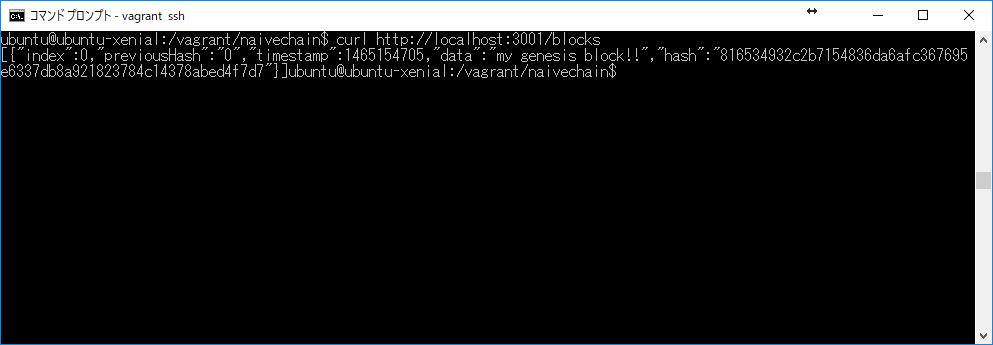
\includegraphics[width=12cm]{images/3001blocks.png}
\caption{NaiveChainでのブロック参照の結果}\label{3001blocks}
\end{figure}
\newpage
\end{enumerate}

\newpage

\subsection{Ethereum}
Ethereum\cite{ethereum}は分散アプリケーションのためのプラットフォームであり,2013年12月以降からオープンソースプロジェクトとして開発が進めれられているものだ.

インターネットの登場以来,メール,SNS,電子決済,クラウド・ファンディングなど数えられないほどのWebサービスを利用して日々を生活している.これらのサービスのほぼ全てにおいて,その運営に何らかの中央管理システムの存在が必須だった.

例えばSNSでは,個人がアップロードしたデータをFacebookやTwitterといった企業は中央で一元管理することでサービスが成り立っている.クラウド・ファインディングでは,Kickstarterのような企業が,資金調達の仲立ちをし,その中で集まった資金についての管理を置こうなうことで,サービスが成り立っている.また,インターネットの基盤であるドメイン名も,ICANNを中心とした管理組織によって管理がなされている.

このような中央管理システムの存在するサービスは以下の点で欠点がある.

\begin{itemize}
\item 可用性:中央管理システムが存在する以上,その中央組織が何らかの理由で潰れなければサービスは継続しない.また,組織が存続している場合でも障害によるデータ消失の危険が避けられない.

\item プライバシー:例えばSNSなど,個人の生活のデータを私的企業が一手に握ることは,データ漏洩の危険性,企業によるデータの不正利用の危険性を考えると好ましいものではない.

\item 検閲:中央の組織により管理されたサービスは,そのサービス提供者による独自の検閲が少なからず入る.検閲するかしないかは「サービス提供者」の手に握られ,たとえそれが公序良俗に「反しない」ものであっても検閲の対象になる可能性がある.
\end{itemize}

Ethereumは「ブロックチェーン」と呼ばれる技術をベースに,なんら特別な管理者のいないP2Pシステム上で様々なサービスを実現するための基盤を提供するものである.つまりFacebookやTwitter,KickstarterやICANNといったような,中央で管理する機関の存在を必要とせずに同様のサービスを実現する基盤を提供している.

\newpage
\subsubsection{Ethereumとは}
ブロックチェーン技術を用いた新たな応用サービス公開するためには,2つの選択肢がある.1つは新たなサービスのために新しいブロックチェーンを構築しそれを使ってサービスを行うこと.2つめは,ビットコインのような既存のブロックチェーンを利用しその上にサービスを構築するというものだ.

新しいブロックチェーンを構築することは,非常に敷居の高い方法だ.実装とテストに相当の工数がかかる.さらに重要なのは,ブロックチェーンを用いた合意形成がサービスの公開当初から安定して動作するためには,事前に相当数の参加者が集まっている必要がある.これは需要の少ないニッチなサービスを展開する際には,非常に致命的な問題となる.

一方で,既存のビットコインのブロックチェーンを利用したサービス提供する場合は,あくまでビットコイン自体の設計上の制限に従う必要があり,非常に不自由なものとなってしまう.

Ethereumは上記のようなブロックチェーンを利用した分散アプリケーションを開発しサービス提供を行う際の障壁を取り除くことを目的とした「分散アプリケーションプラットフォーム」だ.そのプラットフォームを形作るためのプロトコル定義や実装がオープンソース・プロジェクトとして行われている.

Ethereumは独自のP2Pのブロックチェーンネットワークを構築し,分散アプリケーションが動作する実行環境の役割を果たす.様々な分散アプリケーションがEthereumのブロックチェーンを共有して利用することで利用者の少ないニッチな分散アプリケーションでも,ブロックチェーンを利用した「合意形成」が安定して動作する環境を提供する.

また,分散アプリケーションのコードは,ブロックチェーンに組み込まれプルーフ・オブ・ワークの仕組みにより,改ざん不可能になる.このコードはEthereumネットワークに参加する各ノード上で実行され,その結果の状態もブロックチェーンに組み込まれ,やはり改ざんが不可能になる.

ビットコインはブロックチェーンの技術を用いて悪意のある参加者が参加する可能性のあるP2Pネットワーク上で「取引」を正しく動作させる環境でした.一方でEthereumは,取引だけでなく任意のアプリケーションをこのようなP2Pネットワーク上で正しく動作させることを可能にする環境を提供する.

\newpage

\subsubsection{Ethereumの仕組み}
\subsubsection*{内部通貨:ether}
Ethereumでは「ether」という独自の内部通貨が規定されている.ビットコインと同様,それ自体が価値を持つ通貨としての利用も可能だが,より重要な事はetherがEthereum内で分散アプリケーションやスマート・コントラクトを実行するための「燃料」の役割を果たすということだ.Ethereumは上述のように,このプラットフォーム上で動作する分散アプリケーションに対して任意の処理を可能にしており,それぞれの分散アプリケーションの間でその動作に必要な計算資源の量が異なってくる.そこでEthereumでは,分散アプリケーションを実行するためには,その処理の重さに応じた燃料が必要とすることによって,Ethereum上で動作する分散アプリケーション間での計算資源の割り当ての平等性を確保している.

\subsubsection*{アカウント}
Ethereumには「アカウント」と呼ばれるオブジェクトが既定されている.アカウントは20Byteのアドレス(例:0x4c84598c919d82bfde24cdd13cc41f2aad9c33d3)により参照される.アカウントは主に次の4つのフィールドを持つ.
\begin{itemize}
\item nonce:そのアカウントが送信した累積トランザクション数

\item ether balance:そのアカウントが所有するether量

\item contract code:コントラクト・コード(EOAの場合は空)

\item storage:そのアカウントが保持する任意のデータ
\end{itemize}

このフィールドのデータは,アカウント間でトランザクションが発生することにより変化する.つまり,アカウントの「状態」がトランザクションによって変化していく.
「アカウント」には2つのタイプが存在する.1つは「Externally Owned Account(EOA)」もう一つは「Contract」である.EOAは,我々ユーザにより生成されコントロールされるアカウントである.ユーザの任意のタイミングでトランザクションを生成し,他のEOAへのetherの送金,新しいContractの生成やコントラクト・コードの実行を行う.

一方でContractはEOAはからトランザクションを介して生成される.Contractは一種の自動エージェントであり,EOAが発信するトランザクションをトリガに,コントラクト・コードを実行する.

\newpage

\subsubsection*{トランザクション}
EthereumではEOAから任意のタイミングでトランザクションを送信することで,各アカウントの状態が変化する.EOAがトランザクションを生成しそれをEthereumネットワーク上に送信する.採掘者は受信したトランザクションの正当性をチェックし問題なければ,そのトランザクションの情報とトランザクションの内容に基づいて変化した最新のアカウントの状態をブロックチェーンに埋め込む.トランザクションには主に以下の情報が含まれる.
\begin{itemize}
\item ether送金額
\item 相手先アドレス
\item 送信アカウント署名
\item 任意データ
\item STARTGAS値
\item GASPRICE値
\end{itemize}

最初の3つはビットコインのような暗号通貨のトランザクションと同じで,それぞれ,Ethereumの内部通貨であるetherの送金額と相手のアドレス,そしてトランザクションの送信者がether送金元アドレスの所有者であることを証明するデジタル証明だ.

「任意データ」はトランザクションの相手先がContractである場合に,そのコントラクト・コードに引き渡すデータを格納する.

\newpage

\subsubsection*{トランザクションの処理の流れ}
トランザクションによりどのようにアカウントの状態が変更されていくのか大まかに以下のようになる.
\begin{enumerate}
\item EOAがトランザクションを生成し,Ethereumネットワーク上に送信する.

\item ネットワーク内の採掘者がトランザクションを受信する.

\item 採掘者は,署名の正当性など,受信したトランザクションのデータに問題がないかをチェック.問題がある場合にはエラーとして以降の処理を行わない.

\item 採掘者はトランザクション内のSTARTGAS値とGASPRICE値を参照.「STARTGAS値 * GASPRICE値」の量のetherを,前払い手数料として,トランザクションを送信したアカウントの保有するetherから引く.もしetherの保有量が「STARTGAS値 * GASPRICE値」よりも少なければエラーとして以降の処理を行わない.

\item 残りGAS = STARTGAS値とする.

\item トランザクション・データの大きさ1バイト当たり5gasを残りGASから引く.

\item トランザクション内で指定された相手に対して,指定された額のetherを送金.また「トランザクションの相手」がContractの場合は,Contractの持つコードを実行.

\item 送金額のetherを送金者が保有していない,または,コードを実行中に残りGASがゼロになった場合には,手数料の支払情報のみを残し,元の状態にロールバックさせる.トランザクション実行前の状態から,トランザクション実行のための手数料分だけトランザクションの送信者の保有etherから引き,採掘者の保有額にそれを足した状態を終状態とする.

\item 送金,またはコードの実行が正常に終了し,GASが余っている場合は,その余ったGASをトランザクションの送信者に対して戻す.
\end{enumerate}

\newpage

\subsubsection*{ブロックチェーンと採掘}
ビットコインのシステムで,ブロックチェーンはビットコイン・ネットワーク上で発生したすべてのトランザクションを記録した,誰でも参照可能な公開取引元帳の役割を果たしていた.

Ethereumのブロックチェーンも同様に公開元帳の役割を果たします.ただビットコインの場合とは異なり,Ethereumのアカウントのブロックチェーンには,トランザクションだけでなくEthereumネットワークの全アカウントの最新の状態に関する情報も記録される.

つまり,ブロックチェーンにはトランザクションとアカウントの状態が記録されていき,そのブロックチェーンに書き込まれた状態を「正」とするEthereumネットワーク内の合意が形成されていく.

Ethereumネットワーク内の採掘者は,etherの報酬を目当てに,ブロックの採掘競争を続ける.Ethereumでは,新しいブロックが平均して12秒に1回採掘されるように動的プルーフ・オブ・ワークの難易度を調整されるように設計されている.

Ethereumでは,採掘が成功すると
\begin{itemize}
\item 1採掘あたり固定で5ether.
\item ブロックに含まれる全てのcontractのコードを実行した際に消費したgasに相当するether.
\item ブロックに含んだ1つのUncleブロック当たり1/32 ether.
\end{itemize}
の報酬が採掘者に与えられる.

\newpage

\subsection{Ethereumの導入}
研究において構築するプロトタイプを作成するため,Ethereumの導入を行なう.以下に本研究において利用したソフトウェアのバージョンを掲載する.
\begin{itemize}
\item ホストOS:Windows10 64bit
\item ゲストOS:Ubuntu 16.04LTS 64bit
\item Vagrant 2.0.1
\item VirtualBox 5.2.0
\item rsync 5.5.0
\end{itemize}

\subsubsection{Goの導入}
Ethereumにて用いられるプログラミング言語であるGoを導入する.以下にスクリプトを一覧として記載する.
\begin{verbatim}
sudo add-apt-repository ppa:longsleep/golang-backports
sudo apt-get update
sudo apt-get install golang-go -y
go version
\end{verbatim}

Goの導入が完了すると,\texttt{go version}によって導入されたGoのバージョンが図\ref{go}のように表示される.

\begin{figure}[htb]
\centering
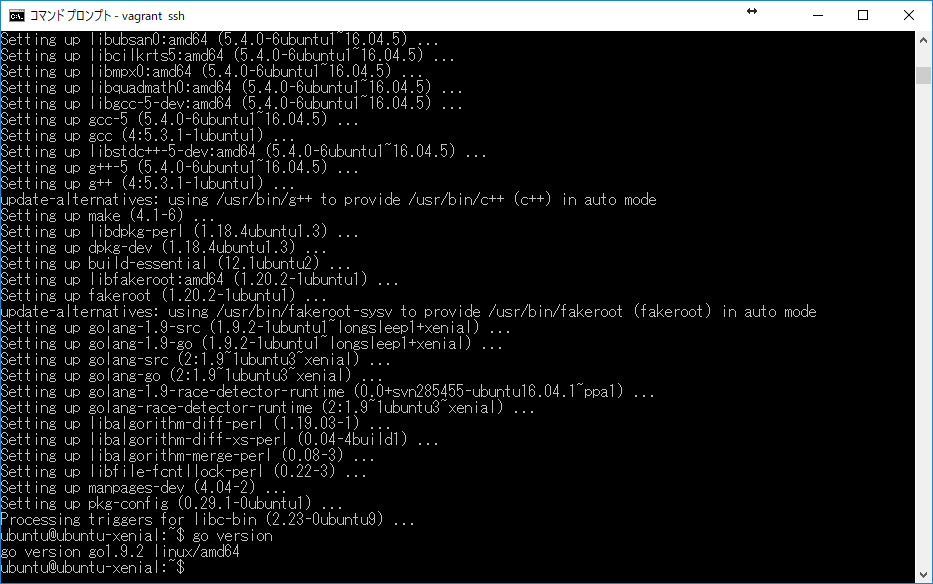
\includegraphics[width=12cm]{images/go.png}
\caption{Goの導入とバージョンの確認}\label{go}
\end{figure}

\subsubsection{Ethereum・Geth・Solcの導入}
Ethereumにて用いられるプラグインのGethとSolcを導入する.以下にスクリプトを一覧として記載する.
\begin{verbatim}
sudo add-apt-repository -y ppa:ethereum/ethereum
sudo apt-get update
sudo apt-get install ethereum -y
sudo apt-get install solc -y
which geth 
which solc
geth version
\end{verbatim}

Geth・Solcの導入が完了すると,\texttt{geth version}によって導入されたGethのバージョンが図\ref{geth}のように表示される.

\begin{figure}[htb]
\centering
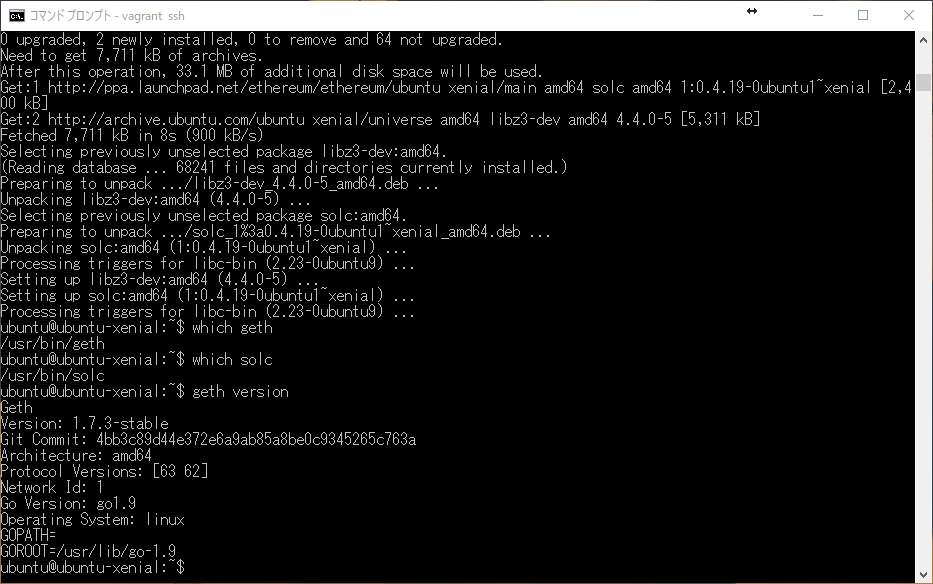
\includegraphics[width=12cm]{images/geth.png}
\caption{Gethの導入とバージョンの確認}\label{geth}
\end{figure}

\newpage

\subsubsection{Gethの起動}
Gethを起動するためには,ローカルプライベートテストネットで次の準備をする必要がある.
\begin{itemize}
\item データディレクトリ
\item Genesisファイル
\end{itemize}
データディレクトリは,送受信したブロックのデータや,アカウント情報を保存するためのディレクトリである.データディレクトリを指定することで,異なるブロックチェーンネットワークを共存させることが出来るようになる.ホームディレクトリにdata\_testnetディレクトリを作成する.
\begin{verbatim}
$ mkdir /data_testnet
$ cd data_testnet
$ pwd
/home/ubuntu/data_testnet 
\end{verbatim}
\texttt{pwd}にて取得したディレクトリは開発において何度も参照することとなるので,控えておくと良い.

続いて「Genesisファイル」を用意する必要がある.Genesisファイルは,ブロックチェーンのGenesisブロック(0番目のブロック)の情報を書いたjson形式のテキストファイルである.同じブロックチェーンネットワークに参加するノードは,同じGenesisブロックから連なるブロックチェーンを共有することとなる.ローカルプライベートネットを構築する場合には,ゼロからブロックチェーンを作ることになるため,Genesisブロックの情報を書いたGenesisファイルが必要となる.先ほど作成したディレクトリにgenesis.jsonを配置する.
\begin{verbatim}
$ vim genesis.json
{
	"config": {},
	"nonce": "0x0000000000000042",
	"timestamp": "0x0",
	"parentHash": "0x000000000000000000000000000000000000000000000000000
0000000000000",
	"gasLimit": "0x8000000",
	"difficulty": "0x4000",
	"mixhash": "0x000000000000000000000000000000000000000000000000000000
0000000000",
	"alloc": {}
}
\end{verbatim}

データディレクトリとGenesisファイルが準備できたら,Gethを初期化する.上記\texttt{pwd}のパスを利用し実行する.
\begin{verbatim}
$ geth --datadir /home/ubuntu/data_testnet init /home/ubuntu/data_testnet/
genesis.json
\end{verbatim}

初期化が完了したらGethを起動する.以降もパスは任意で変更して対応する.問題なく起動すると図\ref{gethup}のようにWelcomeメッセージが表示される.
\begin{verbatim}
$ geth --networkid 4649 --nodiscover --maxpeers 0 --datadir /home/ubuntu/
data_testnet console 2>> home/ubuntu/data_testnet/geth.log
\end{verbatim}
\begin{figure}[htb]
\centering
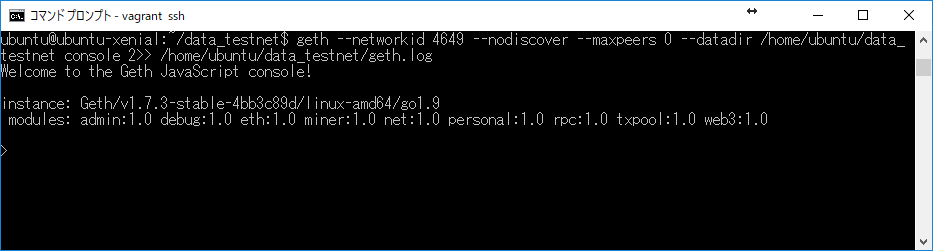
\includegraphics[width=12cm]{images/gethup.png}
\caption{Gethの起動画面}\label{gethup}
\end{figure}
各オプションの意味は以下のとおりである.
\begin{itemize}
\item --networkid 4649

ネットワーク識別子.0から3は予約済みである.(0=Olympic, 1=Frontier, 2=Morden, 3=Ropsten).それ以外の数値であれば問題ない.
\item --nodiscover

利用のノードを,他のノードから検出できないようにするオプションである.ノード追加は手動になる.指定しないと,同じGenesisファイルとネットワークIDのブロックチェーンネットワークに利用中のノードが接続してしまう可能性がある.
\item --maxpeers 0

利用中のノードに接続できるノード数である.0を指定すると,他のノードは接続しなくなる.
\item --datadir /home/ubuntu/data\_testnet

データディレクトリを指定する.指定しないと,ディフォルトのディレクトリが使用される.環境に応じて置き換えて指定する必要がある.
\item console

対話型のJavaScriptコンソールを起動する.
\item 2>> /home/ubuntu/data\_testnet/geth.log

ログファイルを作成するため,エラー処理をリダイレクトする.
\end{itemize}

\chapter{結果}
NaiveChainを用いてブロックの作成と確認を行なうことによって,ブロックチェーンにおけるブロックの繋がりとハッシュ値の関係性について理解を深める.また,Ethereumのテストネットワーク内にてEthereum内の仮想の通貨であるEtherの送金と,研究において構築するプロトタイプの作成を行った結果を記載する.

なお,全スクリプトは執筆時点での内容であり今後のバージョン変更に伴ってスクリプトの訂正が必要となる場合があることをあらかじめ断っておきたい.

\newpage
\section{Naivechainによるブロックの作成}
\ref{addnaivechain}を参照にディレクトリなどを変更したあと,以下の手順で作業を進め,NaiveChainを用いブロック作成を行なうことを通して,ブロックチェーンへの理解を深める.
\begin{enumerate}
\item 新規ブロックを追加するため\texttt{curl -H "Content-type:application/json" 
--data '{"data" : "Some data to the first block"}' http://localhost
:3001/mineBlock}を実行する.その後,再度\texttt{curl http://localhost:3001/blocks}を実行し,作成済みブロックの一覧を表示する.図\ref{mineblocks}のように"index":"1"を含んだ2つ目のブロックが作成されていることを確認する.
\begin{figure}[htb]
\centering
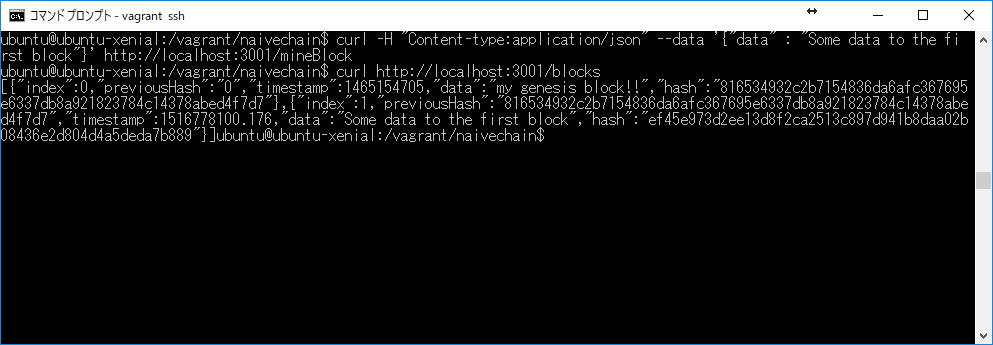
\includegraphics[width=12cm]{images/3001mine.png}
\caption{2つ目のブロックを作成した結果}\label{mineblocks}
\end{figure}
\item もうひとつブロックを追加するため\texttt{curl -H "Content-type:application/json"
--data '{"data" : "Some data to the second block"}' http://localhost
:3001/mineBlock}を実行する.その後,再度\texttt{curl http://localhost:3001/blocks}を実行し,作成済みブロックの一覧を表示する.図\ref{mineblocks2}のように"index":"2"を含んだ3つ目のブロックが作成されていることを確認する.
\begin{figure}[htb]
\centering
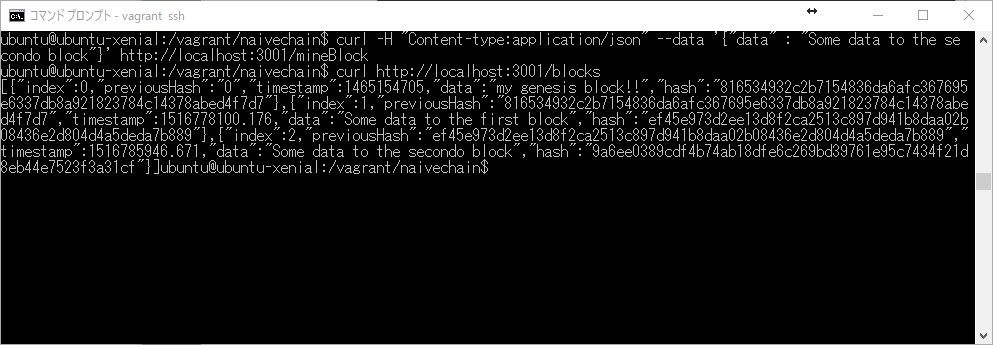
\includegraphics[width=12cm]{images/3001mine2.png}
\caption{3つ目のブロックを作成した結果}\label{mineblocks2}
\end{figure}
\end{enumerate}

\newpage

\subsubsection{ブロックの構造}

まず行うべき作業は,ブロックの構造を決めることである.可能な限りシンプルにするため,最低限必要となる,インデックス,タイムスタンプ,データ,ハッシュ値,そして1つ前のブロックのハッシュ値のみを構造に含める.

\begin{verbatim}
class Block {
    constructor(index, previousHash, timestamp, data, hash) {
        this.index = index;
        this.previousHash = previousHash.toString();
        this.timestamp = timestamp;
        this.data = data;
        this.hash = hash.toString();
    }
}
\end{verbatim}

\subsubsection{ブロックのハッシュ}
ブロックはデータの安全性を確保するため,ハッシュ化されている必要があり,SHA-256によってブロック内のコンテントが引き継がれる.

\begin{verbatim}
var calculateHash = (index, previousHash, timestamp, data) => { 
    return CryptoJS.SHA256(index + previousHash + timestamp + data).toString(); 
}; 
\end{verbatim}

\newpage

\subsubsection{ブロックの生成}
ブロックを生成するには,1つ前のブロックのハッシュ値を知っていなければならず,その上でその他必要なコンテンツ(インデックス,ハッシュ値,データ,タイムスタンプ)を作成する.ブロックデータはエンドユーザによって提供される.

\begin{verbatim}
var generateNextBlock = (blockData) => { 
     var previousBlock = getLatestBlock(); 
     var nextIndex = previousBlock.index + 1; 
     var nextTimestamp = new Date().getTime() / 1000; 
     var nextHash = calculateHash(nextIndex, previousBlock.hash,
   nextTimestamp, blockData); 
     return new Block(nextIndex, previousBlock.hash, nextTimestamp,
   blockData, nextHash); 
 }; 
\end{verbatim}

\subsubsection{ブロックの保存}
ブロックチェーンを保存するには,インメモリのJavaScriptの配列が使用される.ブロックチェーンの最初のブロックは常に「ジェネシスブロック」と呼ばれ,ハードコーディングされている.

\begin{verbatim}
 var getGenesisBlock = () => { 
     return new Block(0, "0", 1465154705, "my genesis block!!",
 "816534932c2b7154836da6afc367695e6337db8a921823784c14378abed4f7d7"); 
 }; 
 
 var blockchain = [getGenesisBlock()]; 
\end{verbatim}

\newpage

\subsubsection{ブロックの安全性の確認}
いかなる場合でも,ブロックもしくはブロックのチェーンが安全性を満たしているか確認しなければならない.特に他のノードから新しいブロックを受け取ったときゃ,承認すべきかどうかの決断をしなければならない場合は重要となる.

\begin{verbatim}
 var isValidNewBlock = (newBlock, previousBlock) => { 
     if (previousBlock.index + 1 !== newBlock.index) { 
         console.log('invalid index'); 
         return false; 
     } else if (previousBlock.hash !== newBlock.previousHash) { 
         console.log('invalid previoushash'); 
         return false; 
     } else if (calculateHashForBlock(newBlock) !== newBlock.hash) { 
         console.log('invalid hash: ' + calculateHashForBlock(newBlock) + ' ' 
         + newBlock.hash); 
         return false; 
     } 
     return true; 
 }; 
\end{verbatim}

\subsubsection{最長チェーンを選択}
いかなる場合でも,チェーンには明確なブロックのセットが1つでなくてはならない.矛盾する点があった場合はブロックの数が多いチェーンを選択する.

\begin{verbatim}
 var replaceChain = (newBlocks) => { 
     if (isValidChain(newBlocks) && newBlocks.length > blockchain.length) { 
         console.log('Received blockchain is valid. Replacing current blockchain
          with received blockchain'); 
         blockchain = newBlocks; 
         broadcast(responseLatestMsg()); 
     } else { 
         console.log('Received blockchain invalid'); 
     } 
 }; 
\end{verbatim}

\newpage

\subsubsection{他のノードとの連絡}
ノードに不可欠なのは,ブロックチェーンを他のノードと共有,また同期する点である.以下は,ネットワークが常に同期されるために必要なルールである.

\begin{itemize}
\item ノードが新しいブロックを生成したら,ネットワークへと送信する.
\item ノードが新しいピアに連結したら,最新のブロックに対してクエリを行う.
\item ノードが,最新として知られるブロックのインデックスよりも大きいインデックスのブロックに出くわしたら,最新のチェーンにそのブロックを追加するか,全ブロックチェーンに対してクエリを行う.
\end{itemize}

\subsubsection{ノードの制御}
何らかの方法で,ユーザはノードを制御する必要がある.これはHTTPサーバを設定することで可能である.

\begin{verbatim}
var initHttpServer = () => {
    var app = express();
    app.use(bodyParser.json());
 
    app.get('/blocks', (req, res) => res.send(JSON.stringify(blockchain)));
    app.post('/mineBlock', (req, res) => {
        var newBlock = generateNextBlock(req.body.data);
        addBlock(newBlock);
        broadcast(responseLatestMsg());
        console.log('block added: ' + JSON.stringify(newBlock));
        res.send();
    });
    app.get('/peers', (req, res) => {
        res.send(sockets.map(s => s._socket.remoteAddress + ':' 
        + s._socket.remotePort));
    });
    app.post('/addPeer', (req, res) => {
        connectToPeers([req.body.peer]);
        res.send();
    });
    app.listen(http_port, () => console.log('Listening http on port: '
   + http_port));
};
\end{verbatim}

\newpage

以下の方法で,ユーザはノードとの情報交換が可能となる.

\begin{itemize}
\item 全てのブロックを記載する.
\item ユーザから与えられたコンテントを基に新しいブロックを作成する.
\item ピアを記載するか追加する.
\end{itemize}

\begin{figure}[htb]
\centering
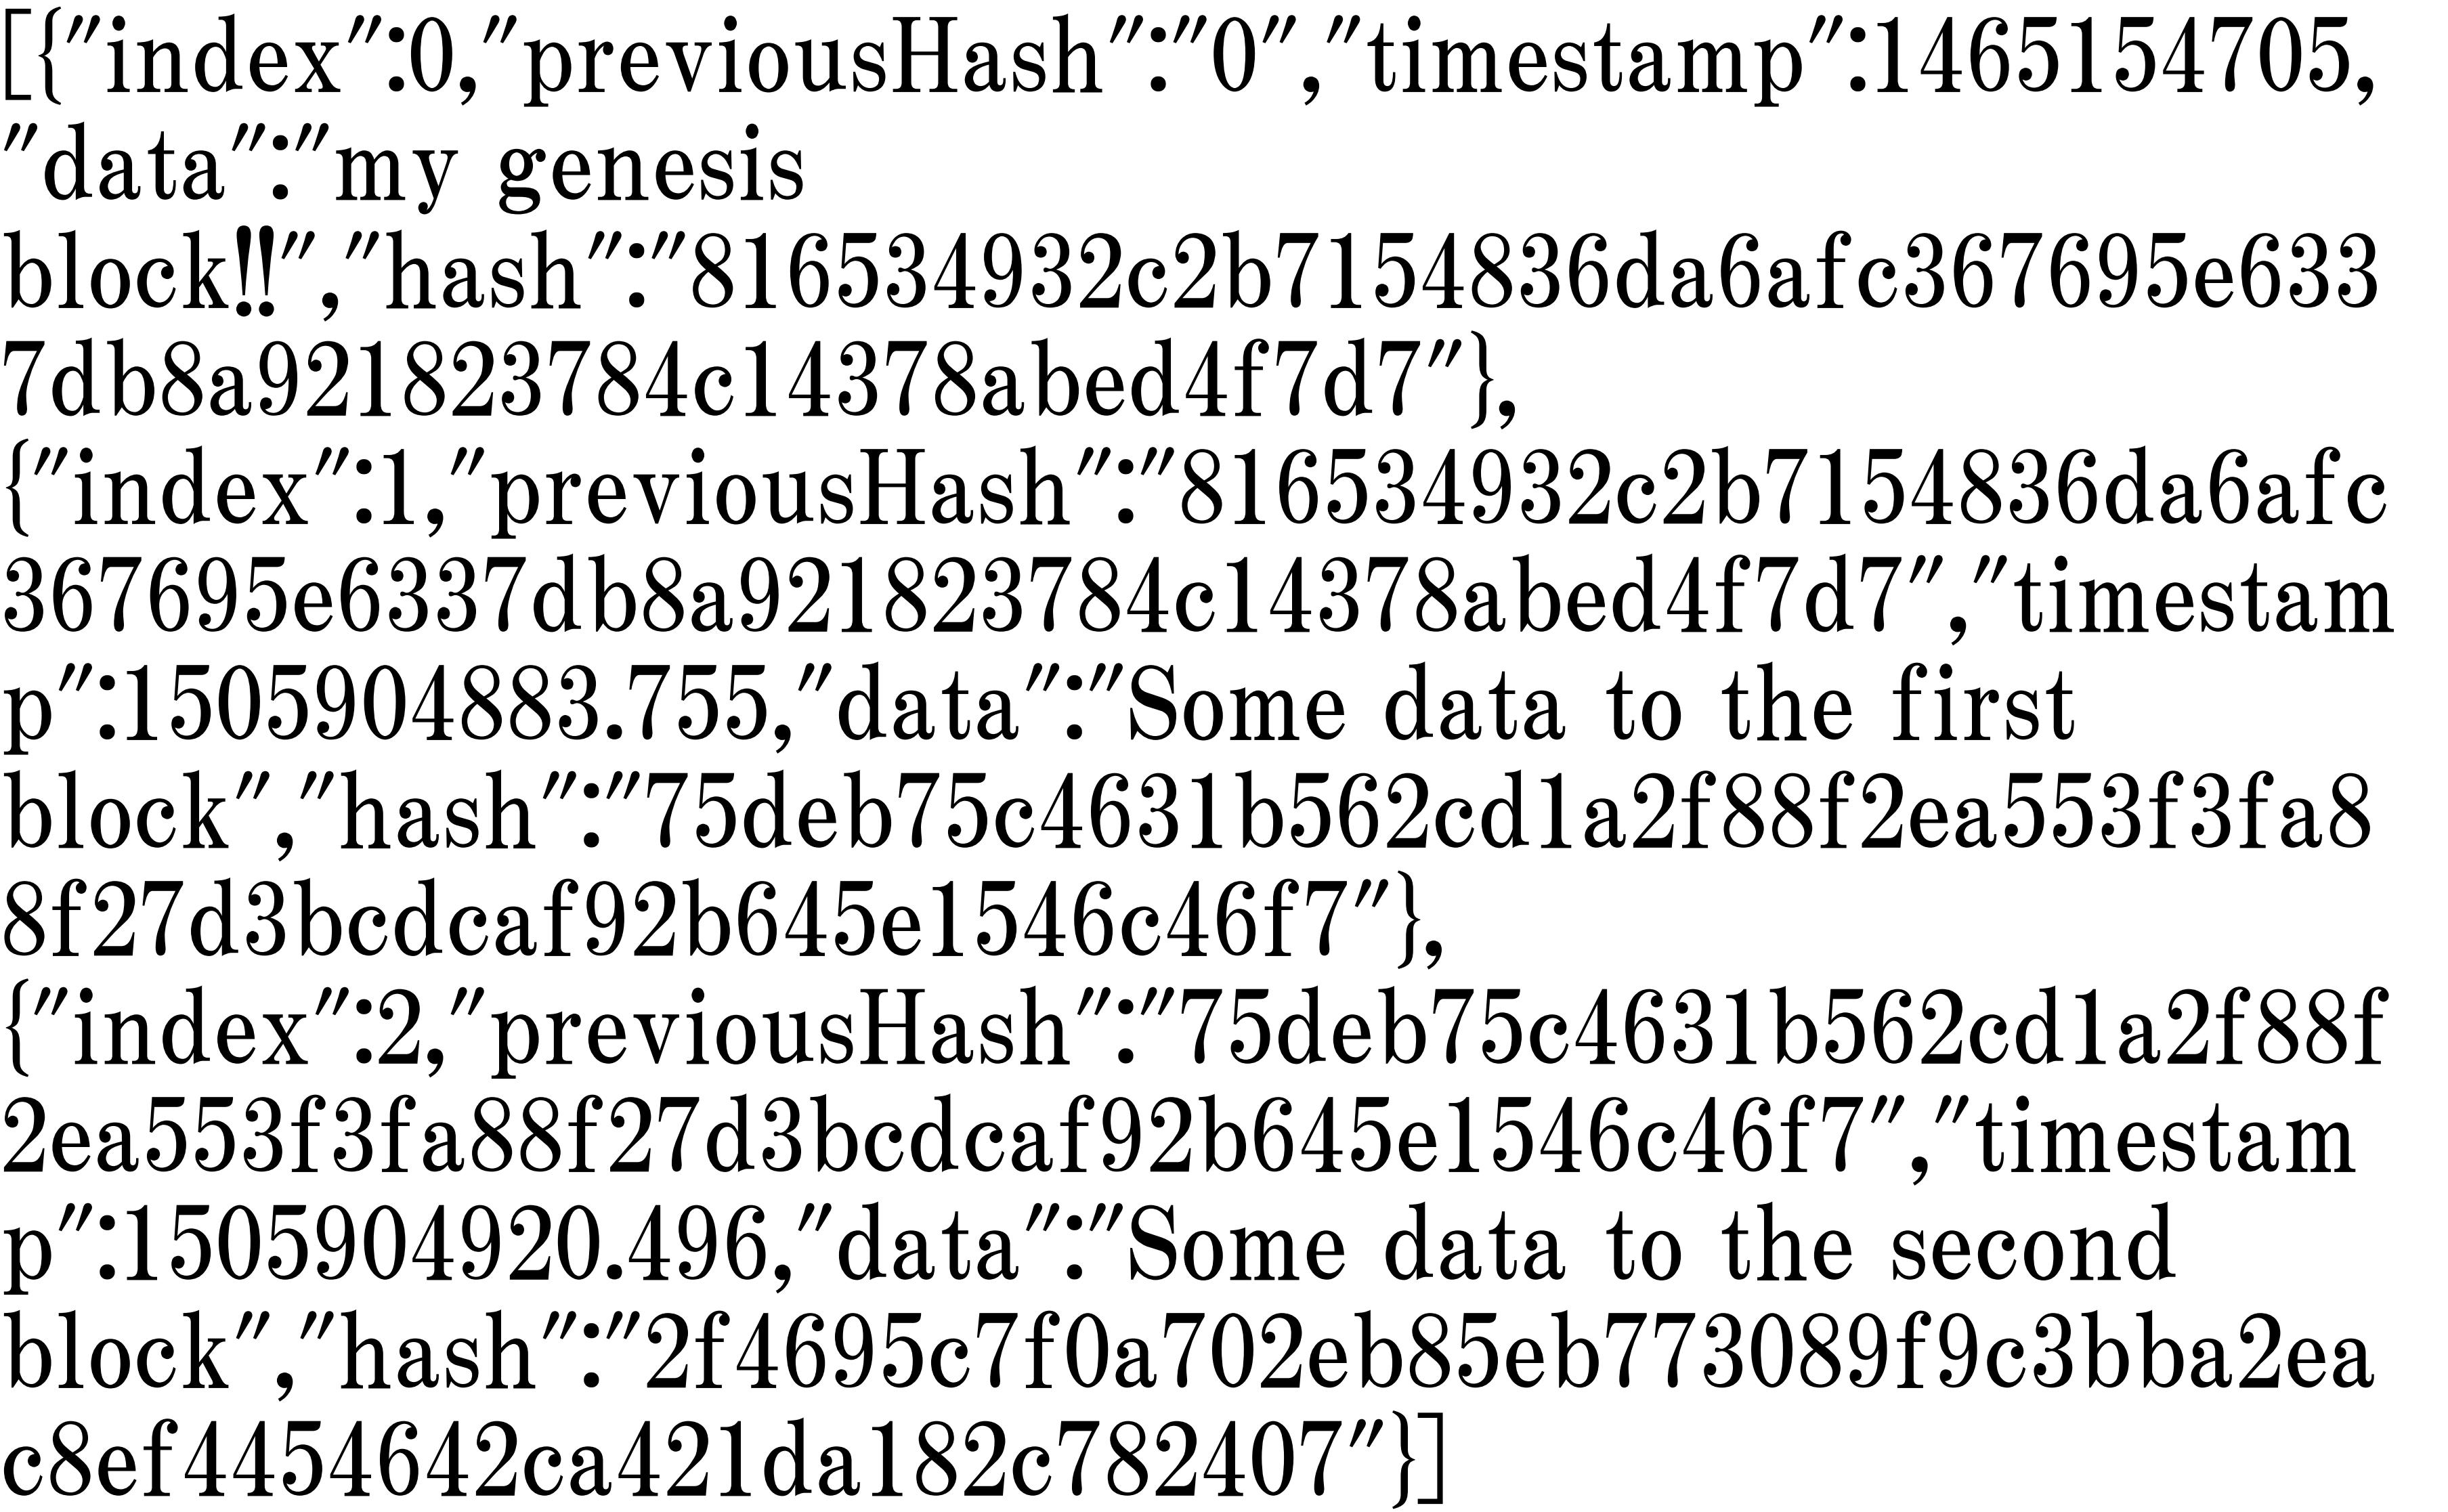
\includegraphics[width=12cm]{images/chaincode.jpg}
\caption{NaiveChainを用いたブロック作成の実行結果}\label{chaincode}
\end{figure}

\begin{figure}[htb]
\centering
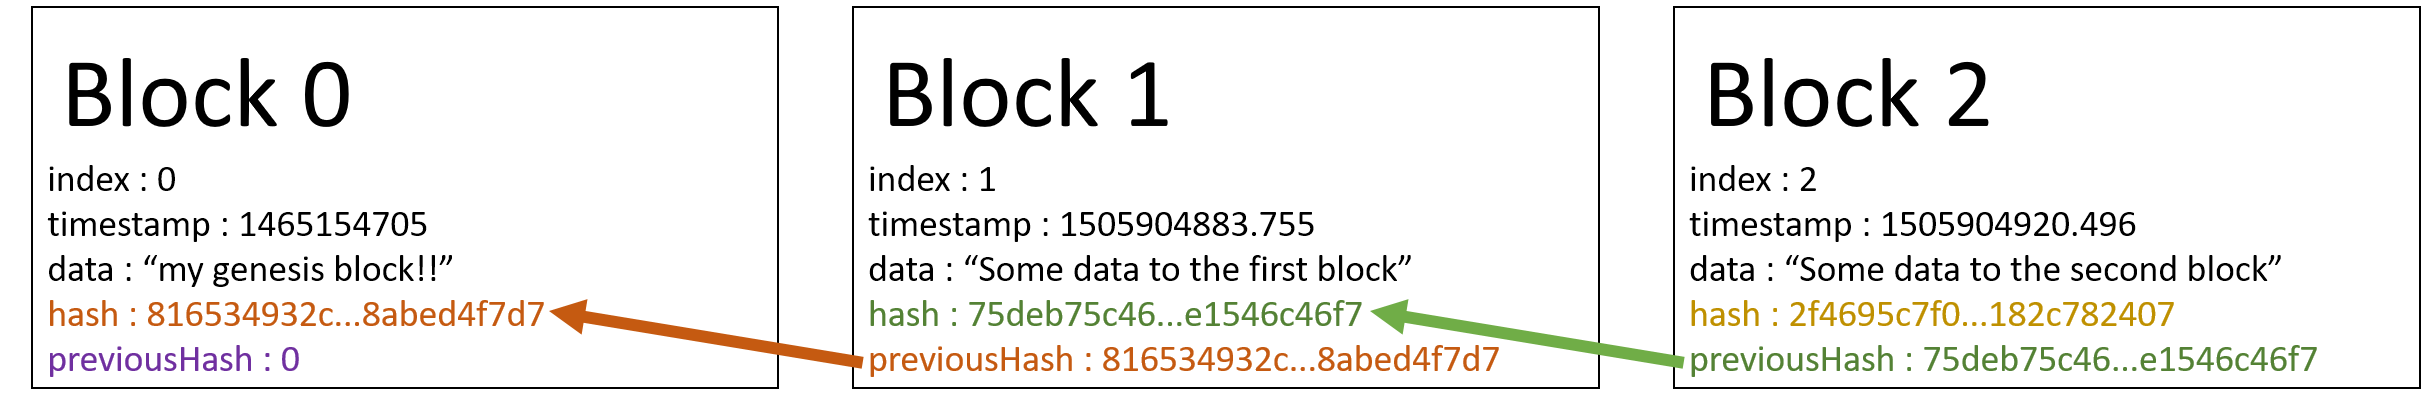
\includegraphics[width=12cm]{images/block.png}
\caption{NaiveChainを用いたブロック作成結果の可視化}\label{block}
\end{figure}

NaiveChianはデモンストレーションおよび学習目的で作成された.このブロックチェーンには「マイニング」アルゴリズムは含まれていないので,パプリックネットワークで使用することはできないが,ブロックチェーンを動かすための基本的な機能は実装されている.図\ref{chaincode}はブロック作成の実行結果.図\ref{block}はその結果を可視化したものである.

\newpage

\section{Ethereumを用いたブロックチェーン環境構築}
\subsection{Etherの送金}
EthereumにはEOAとContractの2種類のアカウントがあることを説明した.今回はEOAを作成する.
\begin{verbatim}
> personal.newAccount("pass0")
"0x37ca4013f17e6fd8062afd8f9f66218d7a5ebfa2"
\end{verbatim}
"pass0"はアカウントノパスフレーズで,半角英数記号を使用した任意の文字列を指定できる.非常に用意なパスフレーズを指定したが,本番環境で使用する際には適切な長さで複雑なパスフレーズを指定する必要がある.ただし,忘れると復元することが出来ない.

"0x37ca4013f17e6fd8062afd8f9f66218d7a5ebfa2"は,作成されたアカウントのアドレスである.このアドレスを指定して送金などを行うことになる.ここで,アドレスはユニークになるように作成されるので,実行の結果は環境によって異なる.アカウントの確認は\texttt{eth.accouns}コマンドで行う.このコマンドで表示されるアドレスは,当該ノードで管理しているアカウントのアドレスとなる.
\begin{verbatim}
> eth.accounts
["0x37ca4013f17e6fd8062afd8f9f66218d7a5ebfa2"]
\end{verbatim}

アカウントの作成が確認できたら,Etherの送金を行うために,もうひとつアカウントを作成する.作成後は\texttt{eth.accounts}コマンドで表示されるアカウントが増えたことを確認する.
\begin{verbatim}
> personal.newAccount("pass1")
"0x8a122d7d3283126ee0e10bb2b9e6b4ddd0a7b32b"
> eth.accounts
["0x37ca4013f17e6fd8062afd8f9f66218d7a5ebfa2", 
"0x8a122d7d3283126ee0e10bb2b9e6b4ddd0a7b32b"]
\end{verbatim}

\texttt{exit}コマンドでGethを終了する.

Gethを起動していない状態でもアカウントを作成することが出来る.パスフレーズはpass2としてアカウントを新規作成してみる.
\begin{verbatim}
$ geth --datadir /home/ubuntu/data_testnet account new
Your new account is locked with a password. Please give a password. 
Do not forget this password.
Passphrase:pass2
Repeat passphrase:pass2
Address: {a92c91ea62cfa0d0a0570d46da51ff589b60b0c9}
\end{verbatim}
\newpage
引き続いてgethコマンドでアカウントを確認してみる.
\begin{verbatim}
$ geth --datadir /home/ubuntu/data_testnet account list
Account #0: {37ca4013f17e6fd8062afd8f9f66218d7a5ebfa2} 
keystore:///home/ubuntu/data_testnet/keystore/UTC--2018-01-25T
02-05-03.861297301Z--37ca4013f17e6fd8062afd8f9f66218d7a5ebfa2
Account #1: {8a122d7d3283126ee0e10bb2b9e6b4ddd0a7b32b} 
keystore:///home/ubuntu/data_testnet/keystore/UTC--2018-01-25T
02-18-08.652245148Z--8a122d7d3283126ee0e10bb2b9e6b4ddd0a7b32b
Account #2: {a92c91ea62cfa0d0a0570d46da51ff589b60b0c9}
keystore:///home/ubuntu/data_testnet/keystore/UTC--2018-01-25T
02-23-55.511872679Z--a92c91ea62cfa0d0a0570d46da51ff589b60b0c9
\end{verbatim}

アカウントの確認が出来たら,再度Gethを起動する起動のコマンドは先ほどと同じものである.

起動が完了したら送金するためのEtherをマイニングしていく.Ethereumでは,マイニング成功時に報酬を受け取るアカウントをEtherbaseと言う.Etherbaseは,ディフォルトでは\texttt{eth.account[0]}が設定されている.\texttt{eth.coinbase}コマンドでEtherbaseを確認することが出来る.
\begin{verbatim}
> eth.coinbase
"0x37ca4013f17e6fd8062afd8f9f66218d7a5ebfa2"
\end{verbatim}
Etherbaseは\texttt{miner.setEtherbase}コマンドで変更できる.
\begin{verbatim}
> miner.setEtherbase(eth.accounts[1])
true
\end{verbatim}
変更ができたことを確認してみる.
\begin{verbatim}
> eth.coinbase
"0x8a122d7d3283126ee0e10bb2b9e6b4ddd0a7b32b"
\end{verbatim}
\texttt{miner.setEtherbase}コマンドで変更できることが確認できたら,以降の作業のため元のアカウントに戻しておく.
\begin{verbatim}
> miner.setEtherbase(eth.accounts[0])
true
> eth.coinbase
"0x37ca4013f17e6fd8062afd8f9f66218d7a5ebfa2"
\end{verbatim}
\newpage
現在のアカウントの残高を確認する.残高の確認は\texttt{eth.getBalance}コマンドで,引数にアカウントノアドレスを渡す.作成直後のアカウントはEtherを所有していないため,今の段階ではどのアカウントでも実行結果は0となる.
\begin{verbatim}
> eth.getBalance(eth.accounts[0])
0
> eth.getBalance(eth.accounts[1])
0
> eth.getBalance(eth.accounts[2])
0
\end{verbatim}

Ethereumもビットコインと同様にマイニングによって仮想通貨Etherを報酬として獲得することができる.マイニングは\texttt{miner.start(threadnum)}コマンドで開始できる.ここでthreadnumはマイニングを行うスレッド数である.

\texttt{eth.accounts[0]}から\texttt{eth.accounts[1]}に10etherを送金してみる.送金は,\texttt{sendTransaction}コマンドで行う.fromに送信元のアドレス,toに送信先のアドレス,valueに送金金額をweiで指定する.
\begin{verbatim}
> eth.sendTransaction({from: eth.accounts[0], to: eth.accounts[1], 
value: web3.toWei(10, "ether")})
Error: authentication needed: password or unlock
    at web3.js:3143:20
    at web3.js:6347:15
    at web3.js:5081:36
    at <anonymous>:1:1
\end{verbatim}
トランザクションの発行は手数料になるため,誤って実行できないように通常はロックされており,使用時にロックを解除する必要がある.personal.unlockAccountコマンドにアンロックするアカウントのアドレスを指定して実行する.
\begin{verbatim}
> personal.unlockAccount(web3.eth.accounts[0])
Unlock account 0x37ca4013f17e6fd8062afd8f9f66218d7a5ebfa2
Passphrase:
true
\end{verbatim}
アンロックしたら再度sendTransactionを実行する.結果は発行したトランザクションのIDである.環境によって変化するユニークなものなので,本論と異なる場合がある.
\begin{verbatim}
> eth.sendTransaction({from: eth.accounts[0], to: eth.accounts[1], 
value: web3.toWei(10, "ether")})
"0x1033cb280d6953f68d8ca13df285e8ca21a4f52fb4a4ec0190d4
b136b6566dc2"
\end{verbatim}
\newpage
sendTransactionを実行しただけでは,処理は実行されない.ブロックチェーンでは,ブロックの中にそのトランザクションが取り込まれるときに,トランザクションの内容が実行される.トランザクションの状態を確認してみると,blockNumberがnullとなっている.ブロックにはいっていない,つまり未処理であることが\texttt{eth.pendingTransaction}コマンドで図\ref{pending}のように確認することが出来る.
\begin{figure}[htb]
\centering
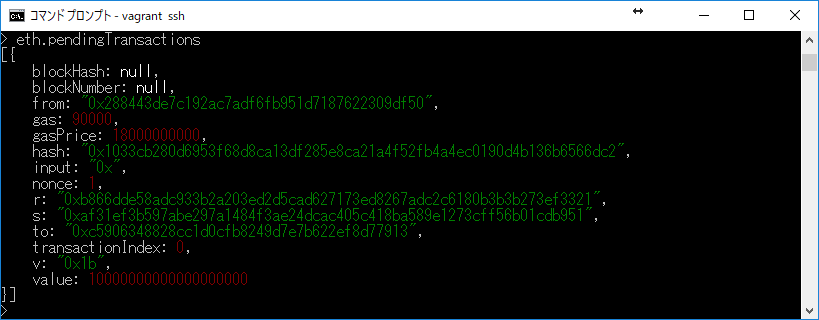
\includegraphics[width=12cm]{images/pending.png}
\caption{ブロックに入っていない未処理のトランザクションを表示した結果}\label{pending}
\end{figure}

\texttt{miner.start}コマンドでマイニングを再開して新しくブロックを作成する.\texttt{eth.pendingTransactions}を実行してトランザクションが表示されなくなったことを確認したら\texttt{eth.getTransaction}コマンドでトランザクションを確認する.先ほどはblockNumberがnullであったが値が追加されていることが図\ref{gettransaction}のように確認できる.
\begin{verbatim}
> miner.start()
null
> eth.pendingTransactions
[ ]
>miner.stop()
true
\end{verbatim}
\begin{figure}[htb]
\centering
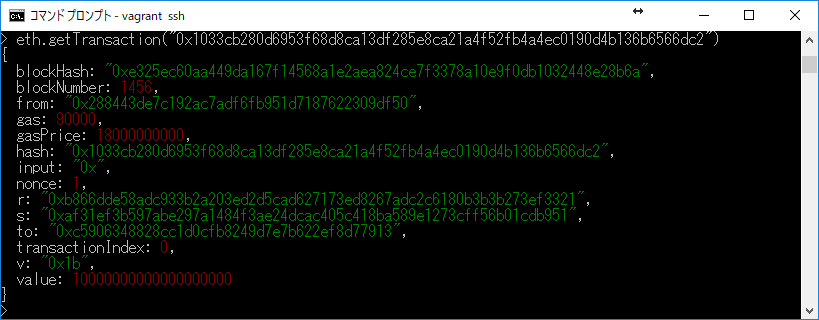
\includegraphics[width=12cm]{images/gettransaction.png}
\caption{ブロックを新たに追加することに成功した結果}\label{gettransaction}
\end{figure}



\newpage
\subsection{スマート・コントラクト}\label{smart}
\subsubsection{スマート・コントラクトの説明}
スマート・コントラクトは,ブロックチェーン上で動作するアプリケーションの位置づけとなる.スマート・コントラクトの開発の大きな流れは,Webアプリケーション開発と同様である.開発者はコードを書き,サーバ(ブロックチェーン)にデプロイする.ユーザはブラウザでサーバにアクセスし,目的の処理を行う.

開発者は高レベルの言語でコントラクトを記述する.そしてそれをEVMコンパイラでコンパイルしてEVMバイトコードにし,ブロックチェーンにデプロイする(EVMとはEthereum Virtual Machineの略).EVMバイトコードは,個々のEVM上で実行される.これはちょうどJavaプログラム,Javaバイトコード,JVMの関係に似ている.なお「ブロックチェーンにデプロイする」とは,ブロック内にEVMバイトコードを保存することを意味する.ブロックチェーンネットワークに参加する全ノードは同じブロックを保持するので,全ノードがEVMバイトコードを保持して実行できることになる.

Ethereumのコントラクトを書くためのプログラム言語は,現在,次の3種類がある.

\begin{itemize}
\item Solidity

Solidityは,JavaScriptに似た構文を持つ言語で,現時点におけるEthereumのコントラクト開発における主要言語であり,最も人気がある.

\item Serpent

SerpentはPythonに似た構文の言語である.インターネット上の情報はそれほど多くない.

\item LLL(Lisp Like Language)

アセンブリに似た低レベルの言語である.
\end{itemize}

\newpage

\subsubsection{スマート・コントラクトの利用}

開発中の環境においてスマート・コントラクトが利用できることを確認するために,"Hello, World!"などの簡単な文字列を返すだけのコントラクトを実行してみる.プログラムの内容は以下のとおりである.
\begin{lstlisting}[basicstyle=\ttfamily\footnotesize, frame=single]
pragma solidity ^0.4.8;
contract HelloWorld {
  string public greeting;
  function HelloWorld(string _greeting) {
    greeting = _greeting;
  }
  function setGreeting(string _greeting) {
    greeting = _greeting;
  }
  function say() constant returns (string) {
    return greeting;
  }
}
\end{lstlisting}

プログラム内の変数は以下の意味を示す.なお,重要な点のみ示す.
\begin{itemize}
\item コントラクトの宣言:\texttt{contract Hello World \{}

contractでコントラクトを宣言する.コントラクトはJavaなどのオブジェクト指向プログラミング言語のクラスと似ており任意の名前を付けることが出来る.

\item 状態変数の宣言:\texttt{string public greeting;}

コントラクト内で有効な変数を宣言できる.Ethereumでは,これを状態変数と呼ぶ.今回はユーザから渡された文字列を保持する変数greetingを宣言した.
\newpage
\end{itemize}
コントラクト実行は以下の手順で行なう,データ部やトランザクションの内容を全文掲載すると膨大な量となるため一部割愛する.

\begin{enumerate}
\item 任意の場所にコントラクトプログラムを配置し,コントラクトプログラムビルド用のデータを出力する.
\begin{verbatim}
$ solc -o ./ --bin --optimize HelloWorld.sol
$ cat HelloWorld.bin
6060604052341561000f57600080fd5b60405161046d38038061.....
.....61e4c1bf9257fd6542dbf1628bf82a571b89769cc4c11f5be0029
\end{verbatim}
\item コントラクトの情報を取得する.
\begin{verbatim}
$ solc --abi HelloWorld.sol
[{"constant":true,"inputs":[],"name":"say","outputs":[{"name":
"","type":"string"}],"payable":false,"stateMutability":"view",
(割愛)e,"stateMutability":"nonpayable","type":"constructor"}]
\end{verbatim}
\item Gethを起動する.
\begin{verbatim}
$ geth --networkid 4649 --nodiscover --maxpeers 0 --datadir /home/
ubuntu/data_testnet console 2>> /home/ubuntu/data_testnet/geth.log
\end{verbatim}
\item コントラクト登録者のロックを解除する.
\begin{verbatim}
> personal.unlockAccount(eth.accounts[0])
Unlock account 0x288443de7c192ac7adf6fb951d7187622309df50
Passphrase:
true
\end{verbatim}
\item コントラクトをブロックチェーンに登録する.
\begin{verbatim}
> HelloContract = web3.eth.contract([{"constant":true,"inputs":[],
(割愛)se,"stateMutability":"nonpayable","type":"constructor"}]);
\end{verbatim}
\item 0xをデータ部に入れて16進数であることを明確にする.
\begin{verbatim}
> Hello = HelloContract.new({from: eth.accounts[0], data: '0x6060
604052341561000f57600080fd5b60(割愛)161046d380aa7098a17
57fd6542dbf1628bf82a571b89769cc4c11f5be0029', gas: 3000000})
\end{verbatim}
\item マイニングを開始する.
\begin{verbatim}
> miner.start()
null
\end{verbatim}
\newpage
\item コントラクトにアクセスするための変数を定義する.
\begin{verbatim}
> contractObj = eth.contract(Hello.abi).at(Hello.address)
\end{verbatim}
\item コントラクト登録者のロックを解除する.
\begin{verbatim}
> personal.unlockAccount(web3.eth.accounts[0])
Unlock account 0x288443de7c192ac7adf6fb951d7187622309df50
Passphrase:
true
\end{verbatim}
\item setGreetingを実行して呼び出す変数を更新する.
\begin{verbatim}
> Hello.setGreeting.sendTransaction("Hello, Ethereum!", 
{from:eth.accounts[0], gas:1000000})
"0x0d9b04455fa0e7672ad20b9d2698834f18af4c07ed5b
1e9efce3ff0a35b4d8c7"
\end{verbatim}
\item sayを実行して更新されたかを確認する.
\begin{verbatim}
> Hello.say.call()
"Hello, Ethereum!"
\end{verbatim}
\end{enumerate}

スマート・コントラクトがここまで問題なく実行できたら,図\ref{hello}のように自身で設定した変数を呼び出すことが成功している.以降は動作の確認が出来たため,スマート・コントラクトをもちいたプロトタイプ作成を開始した.
\begin{figure}[htb]
\centering
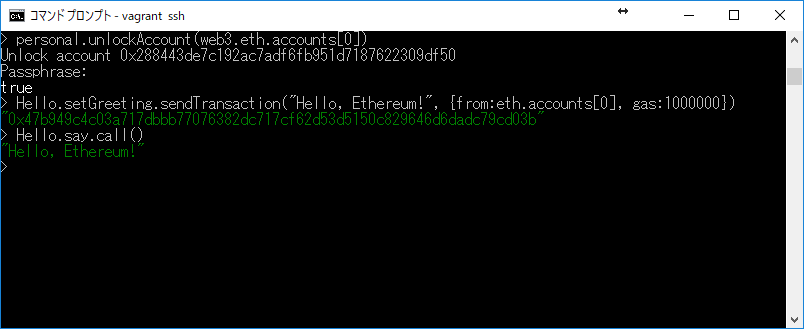
\includegraphics[width=12cm]{images/hello.png}
\caption{スマート・コントラクトをもちいた簡単な変数の設定と出力結果}\label{hello}
\end{figure}
\newpage

\section{プロトタイプモデルの実装}
本研究において,構築したプロトタイプモデルは「出欠情報の管理」「経歴情報の管理」を行なうスマート・コントラクトで実装されたプログラムである.

「出欠情報の管理」を行なうプログラムは,授業およびゼミ等への出席が間違いなく本人によるものであることの証明.授業やゼミが実施された日時において本人が出席していたか欠席していたかの情報の改ざんの防止などを図るために作成したものである.

記録情報は,本人氏名,日時,出欠の有無であり本人氏名と日時を参照することによって出欠情報をブロックチェーンから取り出すことが出来る.

「経歴情報の管理」を行なうプログラムは,記録者本人の所属している研究室や大学,社会人である場合には企業や機関など任意の値を登録することが出来る.記録する本人のアカウントを始め,記録される側のアカウントも作成することによってP2Pネットワークによって本人が間違いなくその組織に所属していることを確認するものである.

記録確認は本人が可能であることはもちろん,閲覧者となる本人以外のアカウントは記録者本人によって閲覧の有無とその期間を決定することができ,ブロックチェーンでの管理のため改ざんの防止も図るよう作成している.

\newpage

\subsection{出欠情報の管理}
任意の値を用いて登録が可能な出欠情報を管理するプログラムを作成した.attendance.solとして作成し,プログラムの内容を以下に記載する.
\begin{lstlisting}[basicstyle=\ttfamily\footnotesize, frame=single]
pragma solidity ^0.4.8;

contract attendance {
    mapping (bytes32 => mapping (bytes32 => string)) public tranlog;

    function setTransaction(bytes32 name, bytes32 date,
 string atten_data) {
        if(bytes(tranlog[name][date]).length != 0) {
            throw;
        }
        tranlog[name][date] = atten_data;
    }

    function getTransaction(bytes32 name, bytes32 date) 
                            constant returns (string atten_data) {
        return tranlog[name][date];
    }
}
\end{lstlisting}

ハッシュ化したnameとdateの他に文字列をatten\_dataとして保存する.setTransactionで任意の値を設定し,getTransactionで情報を取得する.

実行方法は以下に記載するが\ref{smart}と大きく異なる点はない.

\begin{enumerate}
\item 任意の場所にコントラクトプログラムを配置し,コントラクトプログラムビルド用のデータを出力する.
\begin{verbatim}
$ solc -o ./ --bin --optimize attendance.sol
$ cat attendance.bin
6060604052341561000f57600080fd5b60405161046d38038061.....
.....61e4c1bf9257fd6542dbf1628bf82a571b89769cc4c11f5be0029
\end{verbatim}
\item コントラクトの情報を取得する.
\begin{verbatim}
$ solc --abi attendance.sol
[{"constant":true,"inputs":[],"name":"say","outputs":[{"name":
"","type":"string"}],"payable":false,"stateMutability":"view",
(割愛)e,"stateMutability":"nonpayable","type":"constructor"}]
\end{verbatim}
\item Gethを起動する.
\begin{verbatim}
$ geth --networkid 4649 --nodiscover --maxpeers 0 --datadir /home/
ubuntu/data_testnet console 2>> /home/ubuntu/data_testnet/geth.log
\end{verbatim}
\newpage
\item コントラクト登録者のロックを解除する.
\begin{verbatim}
> personal.unlockAccount(eth.accounts[0])
Unlock account 0x288443de7c192ac7adf6fb951d7187622309df50
Passphrase:
true
\end{verbatim}
\item コントラクトをブロックチェーンに登録する.
\begin{verbatim}
> AttenContract = web3.eth.contract([{"constant":true,"inputs":[{
(割愛)payable":false,"stateMutability":"view","type":"function"}]);
\end{verbatim}
\item 0xをデータ部に入れて16進数であることを明確にする.
\begin{verbatim}
> Atten = AttenContract.new({from: eth.accounts[0], data: '0x6060
604052341561000f57600080fd5b60(割愛)161046d380aa7098a17
57fd6542dbf1628bf82a571b89769cc4c11f5be0029', gas: 3000000}, 
function(e, contract){console.log(e, contract); if (typeof contract.
address != 'undefined') { console.log('Contract mined! address: ' + 
contract.address + ' transactionHash: ' + contract.transaction
Hash) ; }})
\end{verbatim}
\item マイニングを開始する.
\begin{verbatim}
> miner.start()
null
> null [object Object]
Contract mined! address: 0x77913d7e41ab1bbae59bf2a0d07492
4f50b01adb transactionHash: 0x0e3cf64b29132e843b23d5591fd
13e0d3684ae897fc09b5ed46b871fa514153a
\end{verbatim}
\newpage
\item コントラクトにアクセスするための変数を定義する.
\begin{verbatim}
> contractObj = eth.contract(Atten.abi).at(Atten.address)
\end{verbatim}
\item コントラクト登録者のロックを解除する.
\begin{verbatim}
> personal.unlockAccount(web3.eth.accounts[0])
Unlock account 0x288443de7c192ac7adf6fb951d7187622309df50
Passphrase:
true
\end{verbatim}
\item setTransactionコマンドを実行し値の設定を行なう.
\begin{verbatim}
> ContractObj.setTransaction.sendTransaction("すずき",
"2018-02-08","出席",{from:eth.accounts[0]})
"0x3dc8b3bcc1cfca430aca271d41da2fd34bb0b41293a782f37d580f9753a1a
770"
\end{verbatim}
\item getTransactionコマンドを実行し,トランザクションの書き込みを確認する.
\begin{verbatim}
> eth.getTransaction("0x3dc8b3bcc1cfca430aca271d41da2fd34bb0b41293a
782f37d580f9753a1a770")
\end{verbatim}
\item callコマンドを実行し,氏名と日時から出欠情報を取り出す.
\begin{verbatim}
> ContractObj.getTransaction.call("すずき","2018-02-08",{form:eth.
accounts[0]})
"出席"
\end{verbatim}
\end{enumerate}

出欠情報の登録が成功すると図\ref{attendance}のようにトランザクションの内容と入力した任意の値が表示される.

\begin{figure}[htb]
\centering
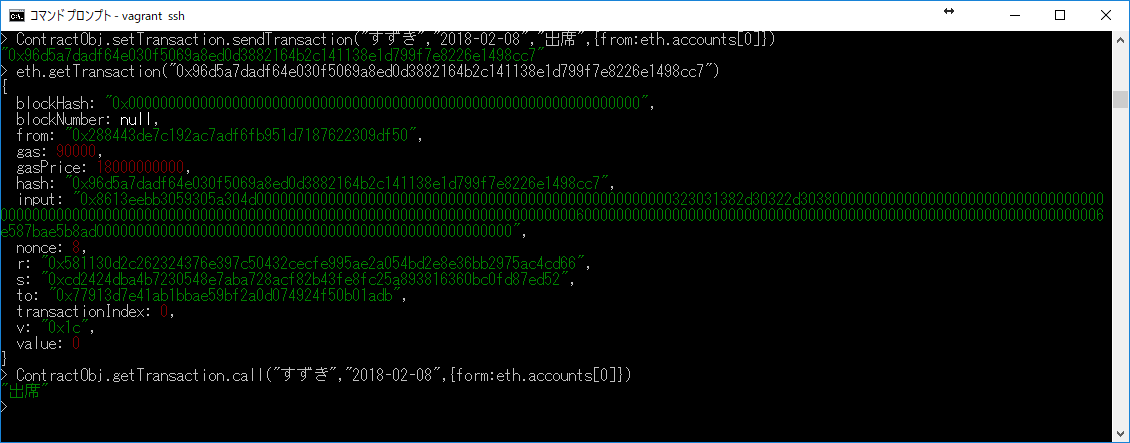
\includegraphics[width=12cm]{images/attendance.png}
\caption{出欠情報を任意で登録し出力の確認を行った結果}\label{attendance}
\end{figure}

\subsection{出欠情報の管理}
任意の値を用いて登録が可能な経歴情報を管理するプログラムを作成した.person.solとして作成し,プログラムの内容を以下に記載する.
\begin{lstlisting}[basicstyle=\ttfamily\footnotesize, frame=single]
pragma solidity ^0.4.8;

contract person {
    address admin;

    struct AppDetail {
        bool allowReference;
        uint256 approveBlockNo;
        uint256 refLimitBlockNo;
        address applicant;
    }

    struct PersonDetail {
        string name;
        string birth;
        address[] orglist;
    }

    struct OrganizationDetail {
        string name;
    }

    mapping(address => AppDetail) appDetail;

    mapping(address => PersonDetail) personDetail;

    mapping(address => OrganizationDetail) public orgDetail;

    function PersonCertification() {
        admin = msg.sender;
    }

    function setPerson(string _name, string _birth) {
        personDetail[msg.sender].name = _name;
        personDetail[msg.sender].birth = _birth;
    }

    function setOrganization(string _name) {
         orgDetail[msg.sender].name = _name;
    }

    function setBelong(address _person) {
        personDetail[_person].orglist.push(msg.sender);
    }

    function setApprove(address _applicant, uint256 _span) {
        appDetail[msg.sender].allowReference = true;
        appDetail[msg.sender].approveBlockNo = block.number;
        appDetail[msg.sender].refLimitBlockNo = block.number + _span;
        appDetail[msg.sender].applicant = _applicant;
    }

    function getPerson(address _person) public constant returns(
                                        bool _allowReference,
                                        uint256 _approveBlockNo,
                                        uint256 _refLimitBlockNo,
                                        address _applicant,
                                        string _name,
                                        string _birth,
                                        address[] _orglist) {
        _allowReference  = appDetail[_person].allowReference;
        _approveBlockNo  = appDetail[_person].approveBlockNo;
        _refLimitBlockNo = appDetail[_person].refLimitBlockNo;
        _applicant       = appDetail[_person].applicant;
        if (((msg.sender == _applicant) 
          && (_allowReference == true) 
          && (block.number < _refLimitBlockNo)) 
         || (msg.sender == admin) 
         || (msg.sender == _person)) {
            _name    = personDetail[_person].name;
            _birth   = personDetail[_person].birth;
            _orglist = personDetail[_person].orglist;
        }
    }
}

\end{lstlisting}
実行方法を以下に記載する.複数のアカウントを用い,異なるアカウントでGethを起動し変数を回すため,コマンドラインの他に並行してTeraTermなどのsshクライアントを用いて作業を行いのが良い.

本論において作成したアカウントを次に一覧としておく.
\begin{itemize}
\item eth.acccounts[0]

0x288443de7c192ac7adf6fb951d7187622309df50
\item eth.acccounts[1]

0xc5906348828cc1d0cfb8249d7e7b622ef8d77913
\item eth.acccounts[2]

0x5d91af951dcf13690ae9448bfa264d91e3c7f740
\item eth.acccounts[3]

0xd4ccd6b5a0b85f2f3bf86a2332968b40c2f91b40
\item eth.acccounts[4]

0xac8952ec60e771e11a484a5ecab9fbfd181d358a
\end{itemize}

\newpage
\begin{enumerate}
\item Contractのアカウントを合計で5つ作成する.パスフレーズとアドレスを忘れないよう記載しておく.
\begin{verbatim}
> personal.newAccount("pass0")
"0x288443de7c192ac7adf6fb951d7187622309df50"
> personal.newAccount("pass1")
"0xc5906348828cc1d0cfb8249d7e7b622ef8d77913"
> personal.newAccount("pass2")
"0x5d91af951dcf13690ae9448bfa264d91e3c7f740"
> personal.newAccount("pass3")
"0xd4ccd6b5a0b85f2f3bf86a2332968b40c2f91b40"
> personal.newAccount("pass4")
"0xac8952ec60e771e11a484a5ecab9fbfd181d358a"
\end{verbatim}
\item コントラクトプログラムビルド用のデータ部を出力する.
\begin{verbatim}
$ solc -o ./ --bin --optimize person.sol
$ cat person.bin
6060604052341561000f57600080fd5b60405161046d38038061.....
.....61e4c1bf9257fd6542dbf1628bf82a571b89769cc4c11f5be0029
\end{verbatim}
\item コントラクトの情報を取得する.
\begin{verbatim}
$ solc --abi person.sol
[{"constant":false,"inputs":[{"name":"_name","type":"string"}],
(割愛)orgDetail","outputs":[{"name":"name","type":"string"}],
"payable":false,"stateMutability":"view","type":"function"}]
\end{verbatim}
\item TeraTermなど外部のsshクライアントからGethを起動する.
\begin{verbatim}
$ geth --datadir /home/ubuntu/data_testnet --networkid 15
 --mine --minerthreads=1 --etherbase=0x288443de7c192a
c7adf6fb951d7187622309df50  --rpc --rpcport 8545 --rpcaddr
 "0.0.0.0" --rpccorsdomain "*" --rpcapi "admin,db,eth,debug,
miner,net,shh,txpool,personal,web3"
\end{verbatim}
\item GethをコマンドラインなどからAttachする.
\begin{verbatim}
$ geth attach rpc:http://localhost:8545 console
\end{verbatim}
\item コントラクトをブロックチェーンに登録する.
\begin{verbatim}
> PersonContract = web3.eth.contract([{"constant":true,"inputs":[{
(割愛)payable":false,"stateMutability":"view","type":"function"}]);
\end{verbatim}
\newpage
\item 0xをデータ部に入れて16進数であることを明確にする.
\begin{verbatim}
> Person = PersonContract.new({from: eth.accounts[0], data: '0x6060
604052341561000f57600080fd5b60(割愛)161046d380aa7098a17
50bc0b06d4acb0fcd2c9575304ae5eade2e4aaf5b', gas: 3000000}, 
function(e, contract){console.log(e, contract); if (typeof contract.
address != 'undefined') { console.log('Contract mined! address: ' + 
contract.address + ' transactionHash: ' + contract.transaction
Hash) ; }})
> null [object Object]
Contract mined! address: 0xaa64c4842108bb6db68e2b88ec8cef54
85e0bfa2 transactionHash: 0xc9ef23f545cb43eb20aca3c0f8d2208
c9197a9c91012f741bd2566f7dea4aa73
\end{verbatim}
\item コントラクトにアクセスするための変数を定義する.
\begin{verbatim}
> contractObj = eth.contract(Person.abi).at(Person.address)
\end{verbatim}
\item eth.accounts[1]でGethを起動する.sshクライアントで実行中のGethを停止し,新たに起動する.コマンドラインでexitする必要はない.
\begin{verbatim}
$ geth --datadir /home/ubuntu/data_testnet --networkid 15
 --mine --minerthreads=1 --etherbase=0xc5906348828cc1
d0cfb8249d7e7b622ef8d77913  --rpc --rpcport 8545 --rpcaddr
 "0.0.0.0" --rpccorsdomain "*" --rpcapi "admin,db,eth,debug,
miner,net,shh,txpool,personal,web3"
\end{verbatim}
\item 組織情報を入力する.
\begin{verbatim}
> personal.unlockAccount(web3.eth.accounts[1])
> contractObj.setOrganization.sendTransaction("chiba institute of
 technology",{from:eth.accounts[1]})
> contractObj.orgDetail.call("0xc5906348828cc1d0cfb8249d7e7b62
2ef8d77913",{from:eth.accounts[1]})
"chiba institute of technology"
\end{verbatim}
\item 記録者が通学していた実績を登録する.
\begin{verbatim}
> contractObjsetBelong.sendTransaction("0xac8952ec60e771e11a
484a5ecab9fbfd181d358a",{from:eth.accounts[1]})
\end{verbatim}
\newpage
\item eth.accounts[2]でGethを起動する.sshクライアントで実行中のGethを停止し,新たに起動する.コマンドラインでexitする必要はない.
\begin{verbatim}
$ geth --datadir /home/ubuntu/data_testnet --networkid 15
 --mine --minerthreads=1 --etherbase=0x5d91af951dcf136
90ae9448bfa264d91e3c7f740  --rpc --rpcport 8545 --rpcaddr
 "0.0.0.0" --rpccorsdomain "*" --rpcapi "admin,db,eth,debug,
miner,net,shh,txpool,personal,web3"
\end{verbatim}
\item 組織情報を入力する.
\begin{verbatim}
> personal.unlockAccount(web3.eth.accounts[2])
> contractObj.setOrganization.sendTransaction("C.I.T Service
",{from:eth.accounts[2]})
> contractObj.orgDetail.call("0x5d91af951dcf13690ae9448bf
a264d91e3c7f740",{from:eth.accounts[2]})
"C.I.T Service"
\end{verbatim}
\item 記録者が通学していた実績を登録する.
\begin{verbatim}
> contractObjsetBelong.sendTransaction("0xac8952ec60e771e11a
484a5ecab9fbfd181d358a",{from:eth.accounts[2]})
\end{verbatim}
\item eth.accounts[4]でGethを起動する.sshクライアントで実行中のGethを停止し,新たに起動する.コマンドラインでexitする必要はない.
\begin{verbatim}
$ geth --datadir /home/ubuntu/data_testnet --networkid 15
 --mine --minerthreads=1 --etherbase=0xac8952ec60e771e
11a484a5ecab9fbfd181d358a  --rpc --rpcport 8545 --rpcaddr
 "0.0.0.0" --rpccorsdomain "*" --rpcapi "admin,db,eth,debug,
miner,net,shh,txpool,personal,web3"
\end{verbatim}
\item 本人情報を登録する.
\begin{verbatim}
> personal.unlockAccount(web3.eth.accounts[4])
> contractObj.setPerson.sendTransaction("Taro YAMADA",
"19850101",{from:eth.accounts[4]})
>contractObj.getPerson.call("0xac8952ec60e771e11a484a5ecab
9fbfd181d358a",{from:eth.accounts[4]})
[false, 0, 0, "0x00000000000000000000000000000000000",
"Taro YAMADA", "19850101",
["0xc5906348828cc1d0cfb8249d7e7b622ef8d77913",
"0x5d91af951dcf13690ae9448bfa264d91e3c7f740"]]
\end{verbatim}
\newpage
\item 記録者が経歴を見る人に閲覧許可を出す.
\begin{verbatim}
> contractObj.setApprove.sendTransaction("0xd4ccd6b5a0b85
f2f3bf86a2332968b40c2f91b40",250,{from:eth.accounts[4], 
gas:3000000})
> contractObj.getPerson.call("0xac8952ec60e771e11a484a5ecab
9fbfd181d358a",{from:eth.accounts[4]})
[true, 1134, 1384, "0xd4ccd6b5a0b85f2f3bf86a2332968b40
c2f91b40","Taro YAMADA", "19850101",
["0xc5906348828cc1d0cfb8249d7e7b622ef8d77913",
"0x5d91af951dcf13690ae9448bfa264d91e3c7f740"]]
\end{verbatim}
\item eth.accounts[3]でGethを起動する.sshクライアントで実行中のGethを停止し,新たに起動する.コマンドラインでexitする必要はない.
\begin{verbatim}
$ geth --datadir /home/ubuntu/data_testnet --networkid 15
 --mine --minerthreads=1 --etherbase=0xd4ccd6b5a0b85f2
f3bf86a2332968b40c2f91b40  --rpc --rpcport 8545 --rpcaddr
 "0.0.0.0" --rpccorsdomain "*" --rpcapi "admin,db,eth,debug,
miner,net,shh,txpool,personal,web3"
\end{verbatim}
\item 本人確認情報を閲覧する.
\begin{verbatim}
> contractObj.getPerson.call("0xac8952ec60e771e11a484a5ecab
9fbfd181d358a",{from:eth.accounts[4]})
[true, 1134, 1384, "0xd4ccd6b5a0b85f2f3bf86a2332968b40
c2f91b40","Taro YAMADA", "19850101",
["0xc5906348828cc1d0cfb8249d7e7b622ef8d77913",
"0x5d91af951dcf13690ae9448bfa264d91e3c7f740"]]
\end{verbatim}

\end{enumerate}

閲覧情報の取得が成功すると図\ref{code}のように表示される.閲覧期限内に情報を取得しようとした場合には,本人の氏名と生年月日が正しく表示される.閲覧期限が切れた場合に情報を取得しようとした場合には確認できないという結果も得ることが出来た.

\begin{figure}[htb]
\centering
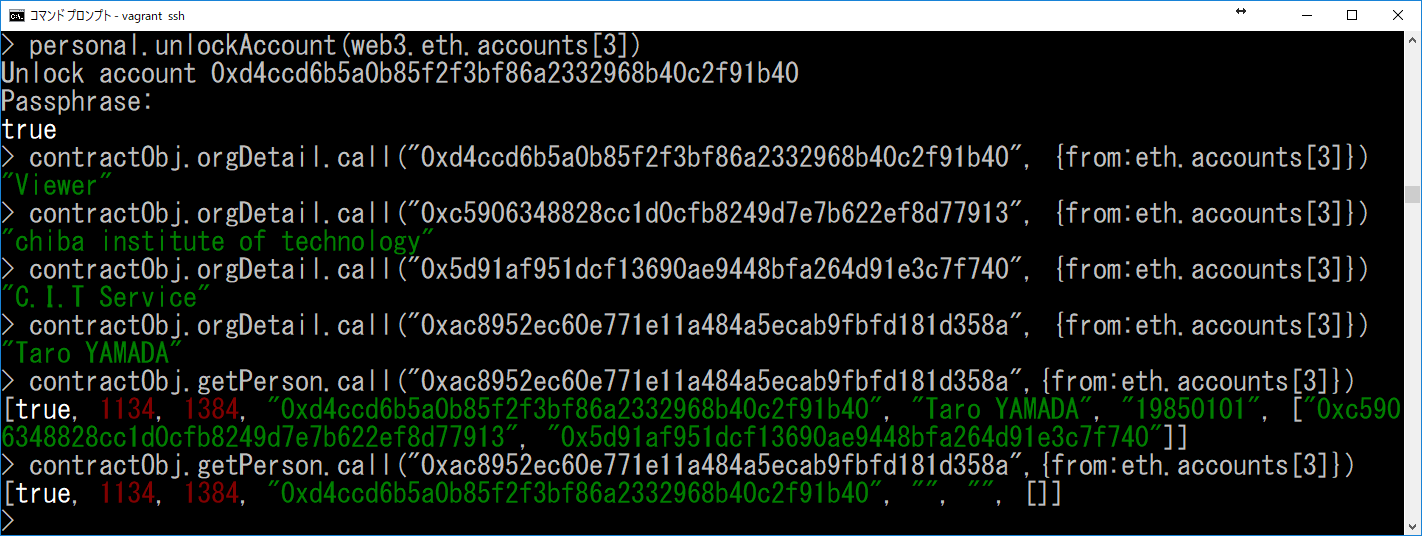
\includegraphics[width=11cm]{images/code.png}
\caption{登録された経歴情報の結果}\label{code}
\end{figure}

\chapter{考察}

ブロックチェーンを用いた存在証明を行なうプログラムをスマート・コントラクトにて構築することが出来た.存在証明が必要となるドキュメントを管理することが多いPM学科内において,幅広く利用する価値があるのではないかと考えた.

電子記録の存在証明はプロジェクト内の成果物において利用することも重要であるため,構築したプロトタイプの強化も有用と考える.

\chapter{結論}

証明が必要となるドキュメントをブロックチェーンで管理することで,改ざんを複雑化しデータの信頼性を向上させることが出来た.

マネジメントに応用する点で独自性が低いため,具体的に利用する内容の検討が必要である.PMBOKなどを参考にしながら存在証明を電子的に行なうべきである成果物やその他の情報を洗い出すことによって,今回作成したプロトタイプモデルの更なる有効的な活用法を見つけることが出来るだろう.

\bibliographystyle{junsrt}
\bibliography{biblio}%「biblio.bib」というファイルが必要.

\chapter*{謝辞}\addcontentsline{toc}{chapter}{謝辞}

本研究を進めるにあたって,ご指導を頂いた卒業論文指導教員の矢吹太朗准教授を始め,プロジェクトマネジメント学科の堀内俊幸教授,下田篤教授,田隈広紀准教授に感謝致します.矢吹准教授には研究外にも多くのことを教えていただきました.

また,研究や日常の情報交流の場を通して多くの知識と方法などを教えていただいた矢吹研究室の皆様,その他本研究や大学生活全体を通してかかわっていただいた皆様にも感謝の意をここに表します.

\end{document}
